\documentclass[aspectratio=169,10pt]{beamer}

% --- Packages ---
\usepackage{graphicx}
\usepackage{booktabs}
\usepackage{amsmath,amssymb}
\usepackage{tikz}
\usetikzlibrary{positioning,arrows.meta,shapes.geometric,shadows,fit,backgrounds}
\usepackage{xcolor}
\usepackage{hyperref}
\usepackage{array}
\usepackage{multicol}
\usepackage{colortbl}
\usepackage{caption}
\captionsetup{font=scriptsize,labelfont=bf}
\usepackage[most]{tcolorbox}

\graphicspath{{assets/flow/}{assets/arch/}{assets/visuals/}{assets/analysis/}{assets/}}

% --- Theme ---
\usetheme{Madrid}
\usecolortheme{whale}
\definecolor{brand}{HTML}{0D3B66}
\definecolor{accent}{HTML}{2A9D8F}
\definecolor{warm}{HTML}{E76F51}
\definecolor{softbg}{HTML}{F4F8FB}
\definecolor{rule}{HTML}{264653}
\setbeamercolor{palette primary}{bg=brand,fg=white}
\setbeamercolor{palette secondary}{bg=accent,fg=white}
\setbeamercolor{frametitle}{bg=brand,fg=white}
\setbeamercolor{title}{fg=brand}
\setbeamercolor{block title}{bg=brand,fg=white}
\setbeamercolor{block title alerted}{bg=warm,fg=white}
\setbeamercolor{block title example}{bg=accent,fg=white}
\setbeamercolor{block body}{bg=softbg}
\setbeamertemplate{navigation symbols}{}
\setbeamertemplate{footline}[frame number]
\setbeamerfont{frametitle}{series=\bfseries}

% --- Metadata ---
\title[Anatomy-Aware CT$\leftrightarrow$MRI Synthesis]{Anatomy-Aware Cross-Modal Medical Image Synthesis}
\subtitle{Rethinking CT$\leftrightarrow$MRI Translation under Imperfect Paired Supervision}
\author{Group 5 \ \ \textperiodcentered\ \ SynthRAD 2023}
\institute{CS 671 --- End-Term Evaluation}
\date{May 2026}

\begin{document}

% ============ TITLE ============
{
\setbeamertemplate{footline}{}
\begin{frame}[plain]
\begin{tikzpicture}[remember picture,overlay]
  \fill[brand] (current page.north west) rectangle ([yshift=-2.6cm]current page.north east);
  \node[anchor=west,text=white,font=\Large\bfseries] at ([xshift=0.9cm,yshift=-1.0cm]current page.north west)
       {Anatomy-Aware Cross-Modal Medical Image Synthesis};
  \node[anchor=west,text=white,font=\normalsize\itshape] at ([xshift=0.9cm,yshift=-1.7cm]current page.north west)
       {Rethinking CT$\leftrightarrow$MRI Translation under Imperfect Paired Supervision};
  \node[anchor=west,text=white!85!brand,font=\footnotesize] at ([xshift=0.9cm,yshift=-2.25cm]current page.north west)
       {CS\,671 \,\textbullet\, End-Term Evaluation \,\textbullet\, SynthRAD\,2023 \,\textbullet\, May 2026};
  \fill[accent] (current page.south west) rectangle ([yshift=0.25cm]current page.south east);
\end{tikzpicture}

\vspace{2.7cm}
\begin{center}
\begin{tcolorbox}[enhanced,colback=softbg,colframe=brand,
  arc=2mm,boxrule=0.6pt,width=0.78\textwidth,
  title={\bfseries Group 5},coltitle=white,colbacktitle=brand,
  fonttitle=\bfseries,halign title=center,
  drop shadow={black!40!white,opacity=0.25}]
\centering
\renewcommand{\arraystretch}{1.25}
\footnotesize
\begin{tabular}{@{}ll@{\hspace{18pt}}ll@{}}
\textbf{B24039} & Md Hasan Raza      & \textbf{B24034} & Varsha Sahithi \\
\textbf{B24299} & Aaditya Rohilla    & \textbf{B24162} & Sarika \\
\textbf{B24301} & Ajender Pal        & \textbf{B24117} & Bhargavi \\
\textbf{B24145} & Siri Chandana      & \textbf{B24047} & Taruna Jassal \\
\end{tabular}
\end{tcolorbox}
\end{center}
\end{frame}
}

% ============ OUTLINE ============
\begin{frame}{Roadmap}
\vspace{2mm}
\footnotesize
\begin{columns}[T]
\begin{column}{0.48\textwidth}
\begin{tcolorbox}[enhanced,colback=softbg,colframe=brand,arc=1.5mm,boxrule=0.5pt,
  title={\scriptsize\bfseries 1\ \ Motivation \& Problem},coltitle=white,colbacktitle=brand]
Clinical asymmetry of CT \& MRI; why ``paired'' data is not truly paired; re-framing the objective.
\end{tcolorbox}\vspace{1.5mm}
\begin{tcolorbox}[enhanced,colback=softbg,colframe=accent,arc=1.5mm,boxrule=0.5pt,
  title={\scriptsize\bfseries 2\ \ Data \& Pipeline},coltitle=white,colbacktitle=accent]
SynthRAD\,2023, patient-wise splits, 2.5D context, intensity normalisation.
\end{tcolorbox}\vspace{1.5mm}
\begin{tcolorbox}[enhanced,colback=softbg,colframe=brand,arc=1.5mm,boxrule=0.5pt,
  title={\scriptsize\bfseries 3\ \ Models (8 in a 2$\times$2$\times$2 design)},coltitle=white,colbacktitle=brand]
Pix2Pix \textbar\ CycleGAN \textbar\ Paired Diffusion \textbar\ Unpaired Cycle-Diffusion.
\end{tcolorbox}
\end{column}
\begin{column}{0.48\textwidth}
\begin{tcolorbox}[enhanced,colback=softbg,colframe=accent,arc=1.5mm,boxrule=0.5pt,
  title={\scriptsize\bfseries 4\ \ Quantitative Results},coltitle=white,colbacktitle=accent]
Test-set metrics, training curves, distribution analysis.
\end{tcolorbox}\vspace{1.5mm}
\begin{tcolorbox}[enhanced,colback=softbg,colframe=brand,arc=1.5mm,boxrule=0.5pt,
  title={\scriptsize\bfseries 5\ \ Ablation Study},coltitle=white,colbacktitle=brand]
Backbone $\times$ Pairing $\times$ Region; main effects \& interactions.
\end{tcolorbox}\vspace{1.5mm}
\begin{tcolorbox}[enhanced,colback=softbg,colframe=accent,arc=1.5mm,boxrule=0.5pt,
  title={\scriptsize\bfseries 6\ \ Qualitative \& Discussion},coltitle=white,colbacktitle=accent]
Brain \& pelvis comparisons; perceptual$\leftrightarrow$pixel trade-off; limitations \& future work.
\end{tcolorbox}
\end{column}
\end{columns}
\end{frame}


% =========================================================================
\section{Clinical Motivation}
% =========================================================================
\begin{frame}{Clinical Motivation: Why CT$\leftrightarrow$MRI Translation?}
\begin{columns}[T]
\begin{column}{0.55\textwidth}
\begin{block}{The clinical asymmetry}
\footnotesize
\begin{itemize}
    \item \textbf{CT}: electron-density (HU) for dose calculation, fast, ionising
    \item \textbf{MRI}: superior soft-tissue contrast, no radiation, slow \& expensive
    \item Many radiotherapy and surgical-planning workflows want \emph{both}
\end{itemize}
\end{block}
\begin{exampleblock}{Why \emph{synthetic} cross-modality is useful}
\footnotesize
\begin{itemize}
    \item MR-only RT planning needs synthetic CT for dose
    \item CT-only triage centres benefit from synthetic MRI for soft-tissue review
    \item Reduced cost, scan-time and radiation burden
\end{itemize}
\end{exampleblock}
\end{column}
\begin{column}{0.42\textwidth}
\begin{block}{SynthRAD 2023 dataset}
\footnotesize
\begin{tabular}{ll}
\toprule
\textbf{Property} & \textbf{Value} \\\midrule
Regions      & Brain, Pelvis \\
Modalities   & CT, MRI (T1/T2) \\
Patients     & 180 (144 train / 36 test) \\
Split        & Patient-wise (no leakage) \\
HU clip      & $[-1000, 1000]$ \\
\bottomrule
\end{tabular}
\end{block}
\begin{alertblock}{Core challenge}
\scriptsize
Non-linear intensity mapping across a large domain gap, with imperfect anatomical correspondence even in ``paired'' scans.
\end{alertblock}
\end{column}
\end{columns}
\end{frame}


% =========================================================================
\section{Problem Statement}
% =========================================================================
\begin{frame}{Problem Statement: ``Paired'' Data Is Not Truly Paired}
\begin{columns}[T]
\begin{column}{0.5\textwidth}
\begin{alertblock}{Sources of mis-pairing in clinical CT--MRI}
\footnotesize
\begin{itemize}
    \item \textbf{Time gap} between acquisitions (hours--weeks)
    \item \textbf{Organ motion}: breathing, peristalsis, cardiac
    \item \textbf{Bladder \& bowel filling} (pelvis)
    \item \textbf{Tumour progression} or post-treatment change
    \item \textbf{Patient repositioning}, scanner-bed bias
    \item \textbf{Fat / oedema} drift
\end{itemize}
\end{alertblock}
\begin{block}{Consequence}
\footnotesize
Pixel-perfect $G:X_{\text{CT}}\!\to\! X_{\text{MR}}$ is \emph{ill-posed}: the target itself drifts between scans.
Strict paired supervision can therefore \emph{over-constrain} learning.
\end{block}
\end{column}
\begin{column}{0.48\textwidth}
\begin{exampleblock}{Re-framing the objective}
\footnotesize
\textit{From} ``predict the exact ground-truth voxel''
\textit{to} ``produce an \textbf{anatomically plausible} translation that is consistent with the source under cycle and perceptual constraints.''
\end{exampleblock}
\begin{block}{Research questions}
\footnotesize
\begin{enumerate}
    \item How much does \textbf{pairing supervision} actually buy under imperfect alignment?
    \item Does a \textbf{distilled latent-diffusion} prior beat GAN backbones at perceptual realism?
    \item Are the resulting trade-offs \textbf{additive} or \textbf{interactive} across backbone $\times$ pairing?
\end{enumerate}
\end{block}
\end{column}
\end{columns}
\end{frame}


% =========================================================================
\begin{frame}{Why Existing Methods Fall Short}
\footnotesize
\begin{columns}[T]
\begin{column}{0.32\textwidth}
\begin{block}{Pix2Pix \tiny(Isola+ '17)}
\begin{itemize}
    \item Strong paired supervision (L1+adv)
    \item Sensitive to mis-alignment $\Rightarrow$ over-smoothed, mode-collapsed outputs
    \item Cannot exploit unpaired archives
\end{itemize}
\end{block}
\end{column}
\begin{column}{0.32\textwidth}
\begin{block}{CycleGAN \tiny(Zhu+ '17)}
\begin{itemize}
    \item Cycle-consistency, no paired data
    \item Weak structural constraints $\Rightarrow$ \emph{anatomy hallucinations}
    \item Mode collapse \& checkerboard artefacts in 2D
\end{itemize}
\end{block}
\end{column}
\begin{column}{0.32\textwidth}
\begin{block}{Vanilla DDPM}
\begin{itemize}
    \item Excellent generative prior
    \item ${\sim}1000$-step sampling: prohibitive for 3D medical volumes
    \item Lacks medical-domain conditioning out-of-the-box
\end{itemize}
\end{block}
\end{column}
\end{columns}

\vspace{1mm}
\begin{exampleblock}{Our contribution}
\textbf{We benchmark \textbf{four paradigms} $\times$ \textbf{two regions} $=$ \textbf{eight models}, then run a research-grade ablation under \emph{patient-wise} evaluation. We use \textbf{SD-Turbo + LoRA} as a one-step latent-diffusion backbone, evaluated against Pix2Pix and CycleGAN, in both \emph{paired} and \emph{cycle} settings.}
\end{exampleblock}
\end{frame}


% =========================================================================
\section{Dataset \& Pipeline}
% =========================================================================
\begin{frame}{Dataset \& Engineering Pipeline}
\begin{center}
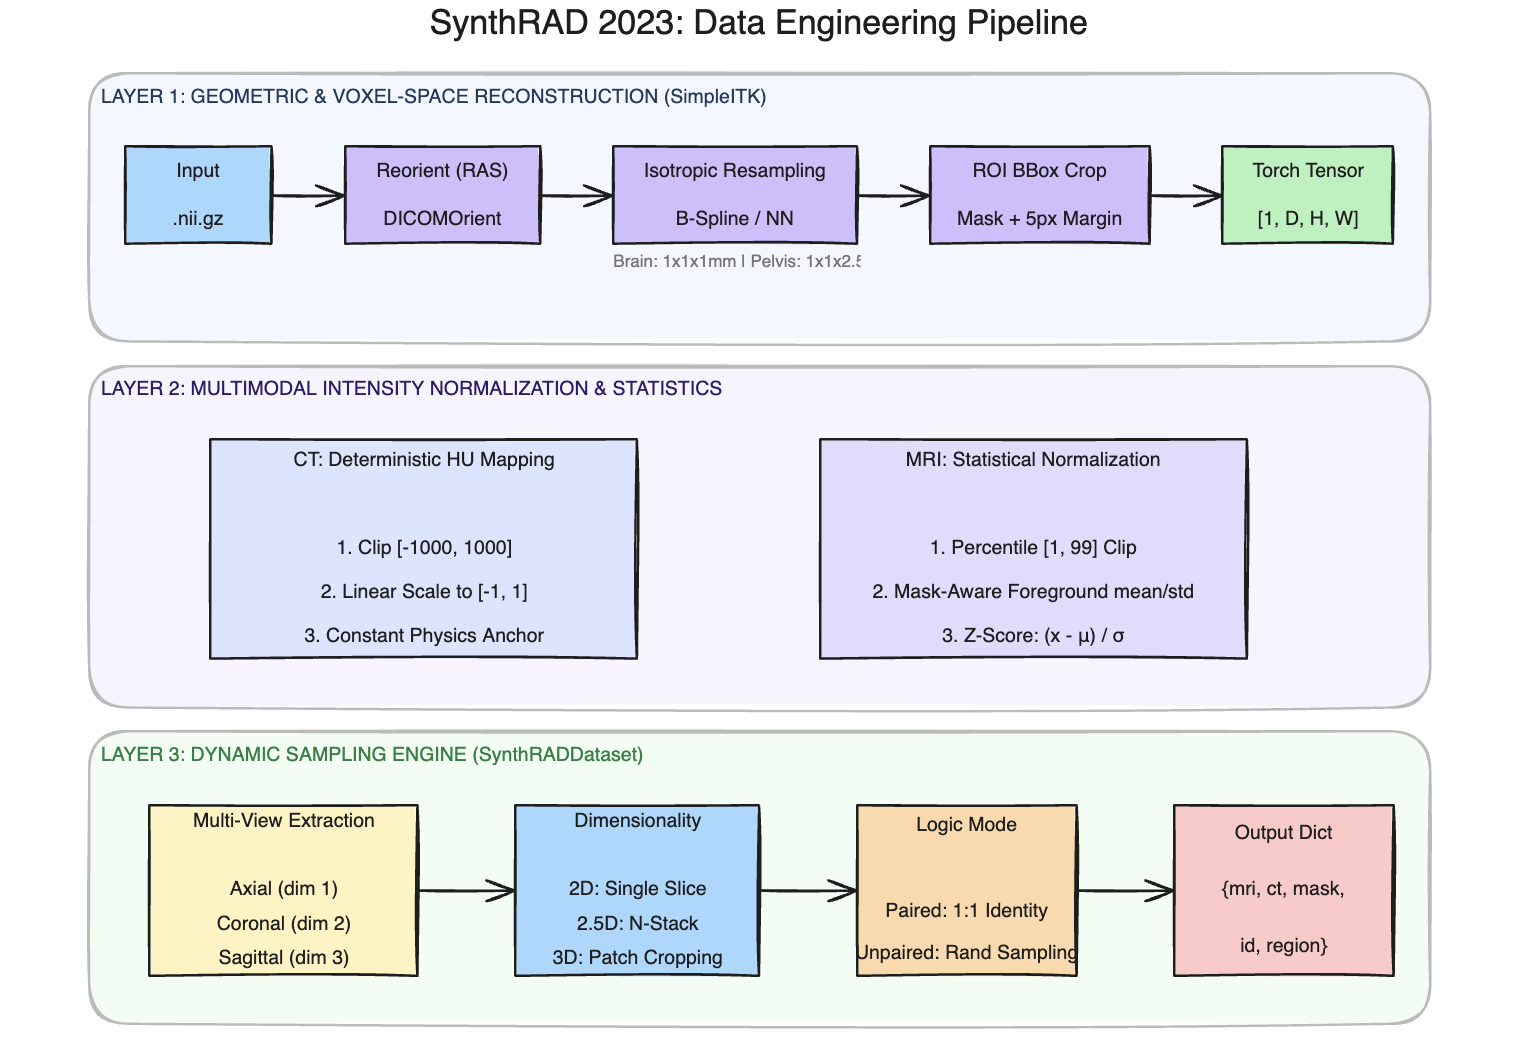
\includegraphics[width=0.62\textwidth,keepaspectratio]{synthrad_data_engineering_pipeline.png}
\end{center}
\vspace{-1mm}
\footnotesize
NIfTI ingestion $\to$ RAS reorient $\to$ resample $\to$ mask-guided crop $\to$ intensity normalisation $\to$ 2D / 2.5D slice sampling $\to$ augmentation $\to$ trainer-specific tensor cache.
\end{frame}


\begin{frame}{Preprocessing Workflow \& Splits}
\begin{columns}[T]
\begin{column}{0.55\textwidth}
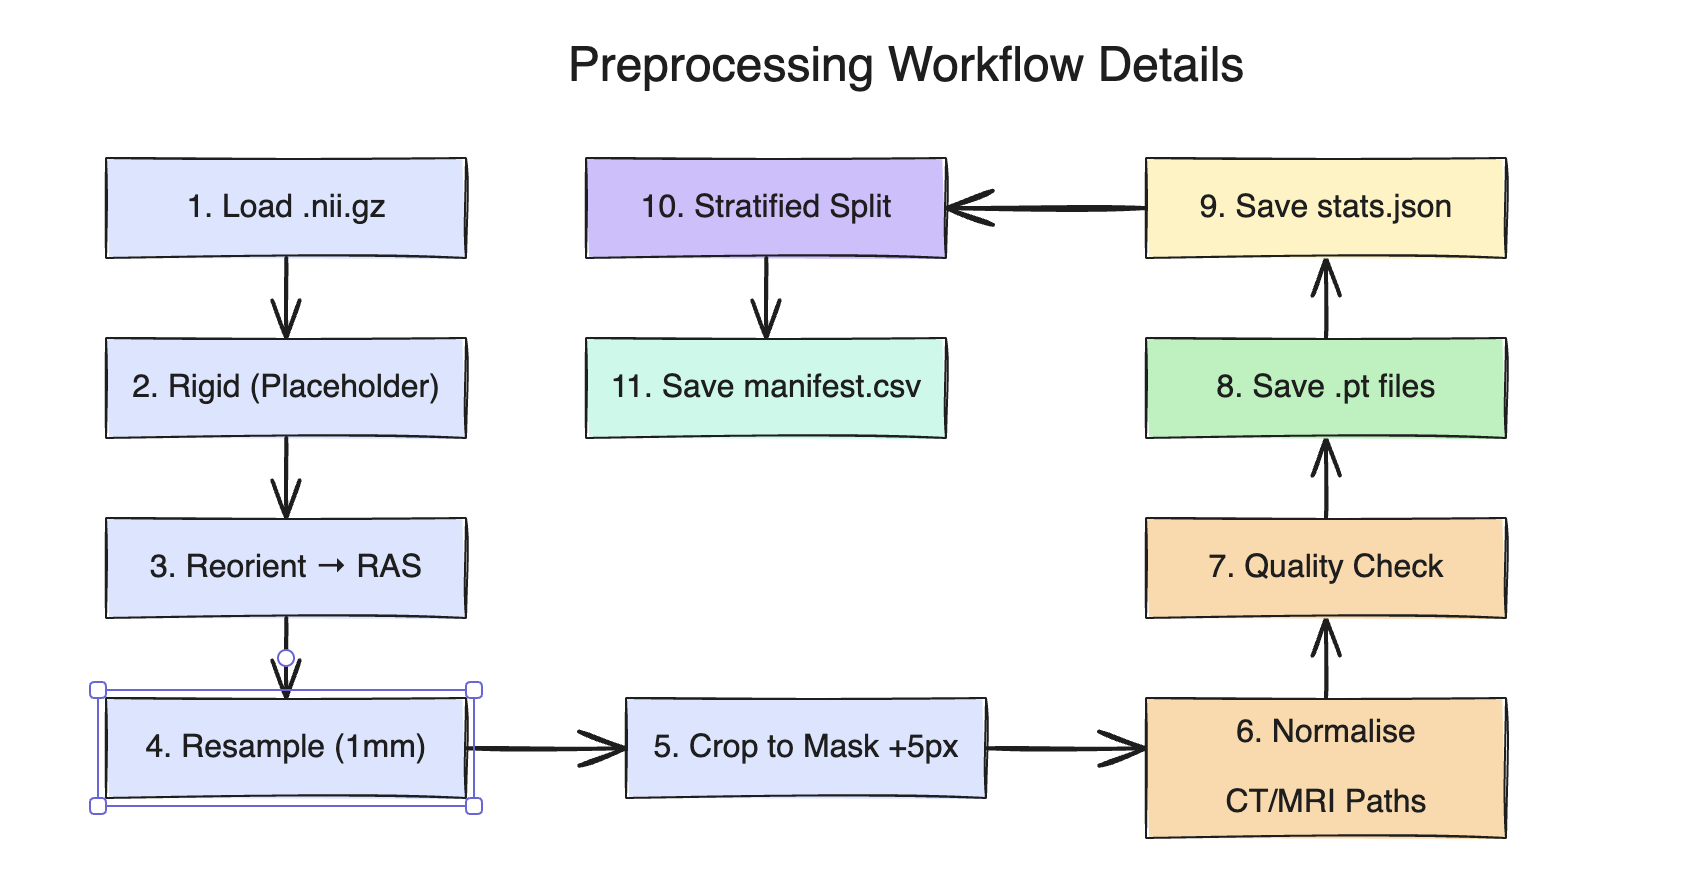
\includegraphics[width=\textwidth]{preprocessing_workflow_details.png}
\end{column}
\begin{column}{0.42\textwidth}
\begin{block}{Patient-wise split (\emph{no leakage})}
\footnotesize
\begin{itemize}
    \item 144 train / 36 test patients
    \item All slices of a patient are in the \emph{same} fold
    \item Slice-wise splits inflate metrics by $\sim$15--30\,\% via memorisation
\end{itemize}
\end{block}
\begin{alertblock}{Resolution choice}
\scriptsize
GANs at $256^{2}$, diffusion at $512^{2}$ to match SD-Turbo's pre-trained manifold. Higher resolution preserves small lesions.
\end{alertblock}
\end{column}
\end{columns}
\end{frame}


\begin{frame}{Intensity Normalisation \& 2.5D Sampling}
\begin{columns}[T]
\begin{column}{0.5\textwidth}
\begin{center}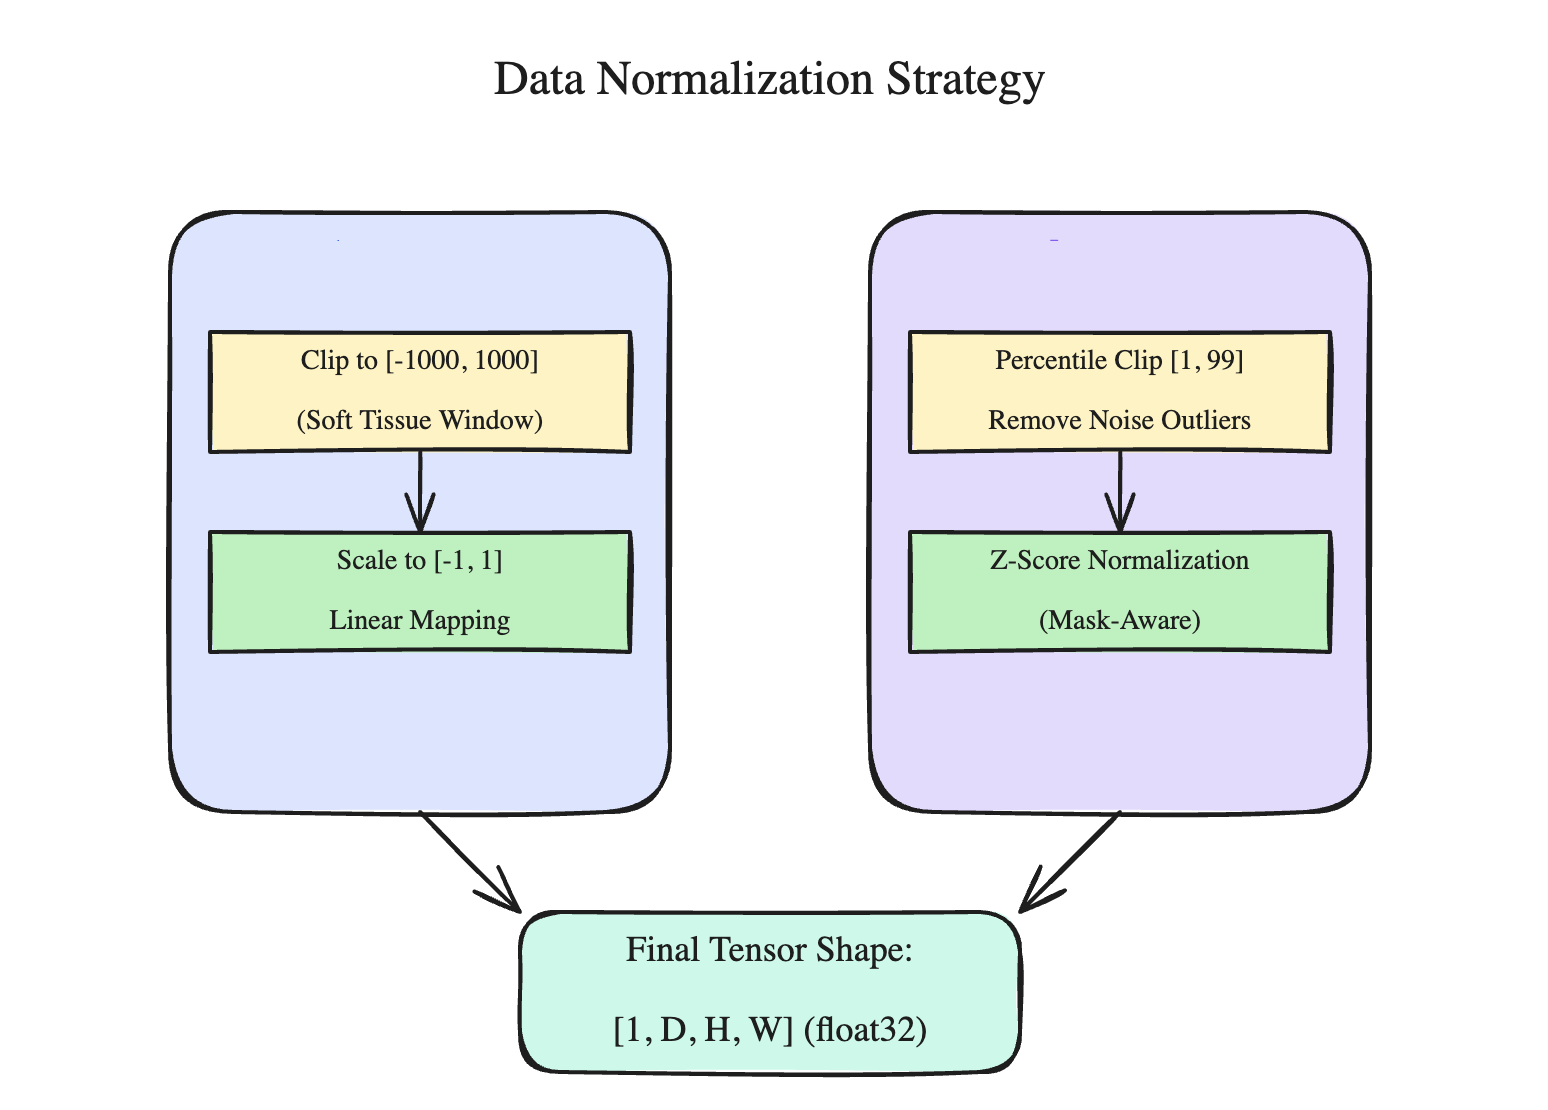
\includegraphics[width=\textwidth]{data_normalization_strategy.png}\end{center}
\end{column}
\begin{column}{0.48\textwidth}
\begin{block}{2.5D context}
\footnotesize
\begin{itemize}
    \item 3 adjacent axial slices stacked into the channel dim
    \item Preserves through-plane anatomical coherence
    \item ${\sim}3{\times}$ cheaper than full 3D, much closer to anatomical reality than pure 2D
\end{itemize}
\end{block}
\begin{block}{Tissue windowing}
\footnotesize
\begin{itemize}
    \item Brain CT: standard brain window before $[-1,1]$ mapping
    \item Pelvis MRI: percentile clip $[1\%, 99\%]$ + foreground Z-score
    \item Soft-tissue windowing essential -- otherwise anatomy invisible
\end{itemize}
\end{block}
\end{column}
\end{columns}
\end{frame}


\begin{frame}{Dataloader Logic}
\begin{center}
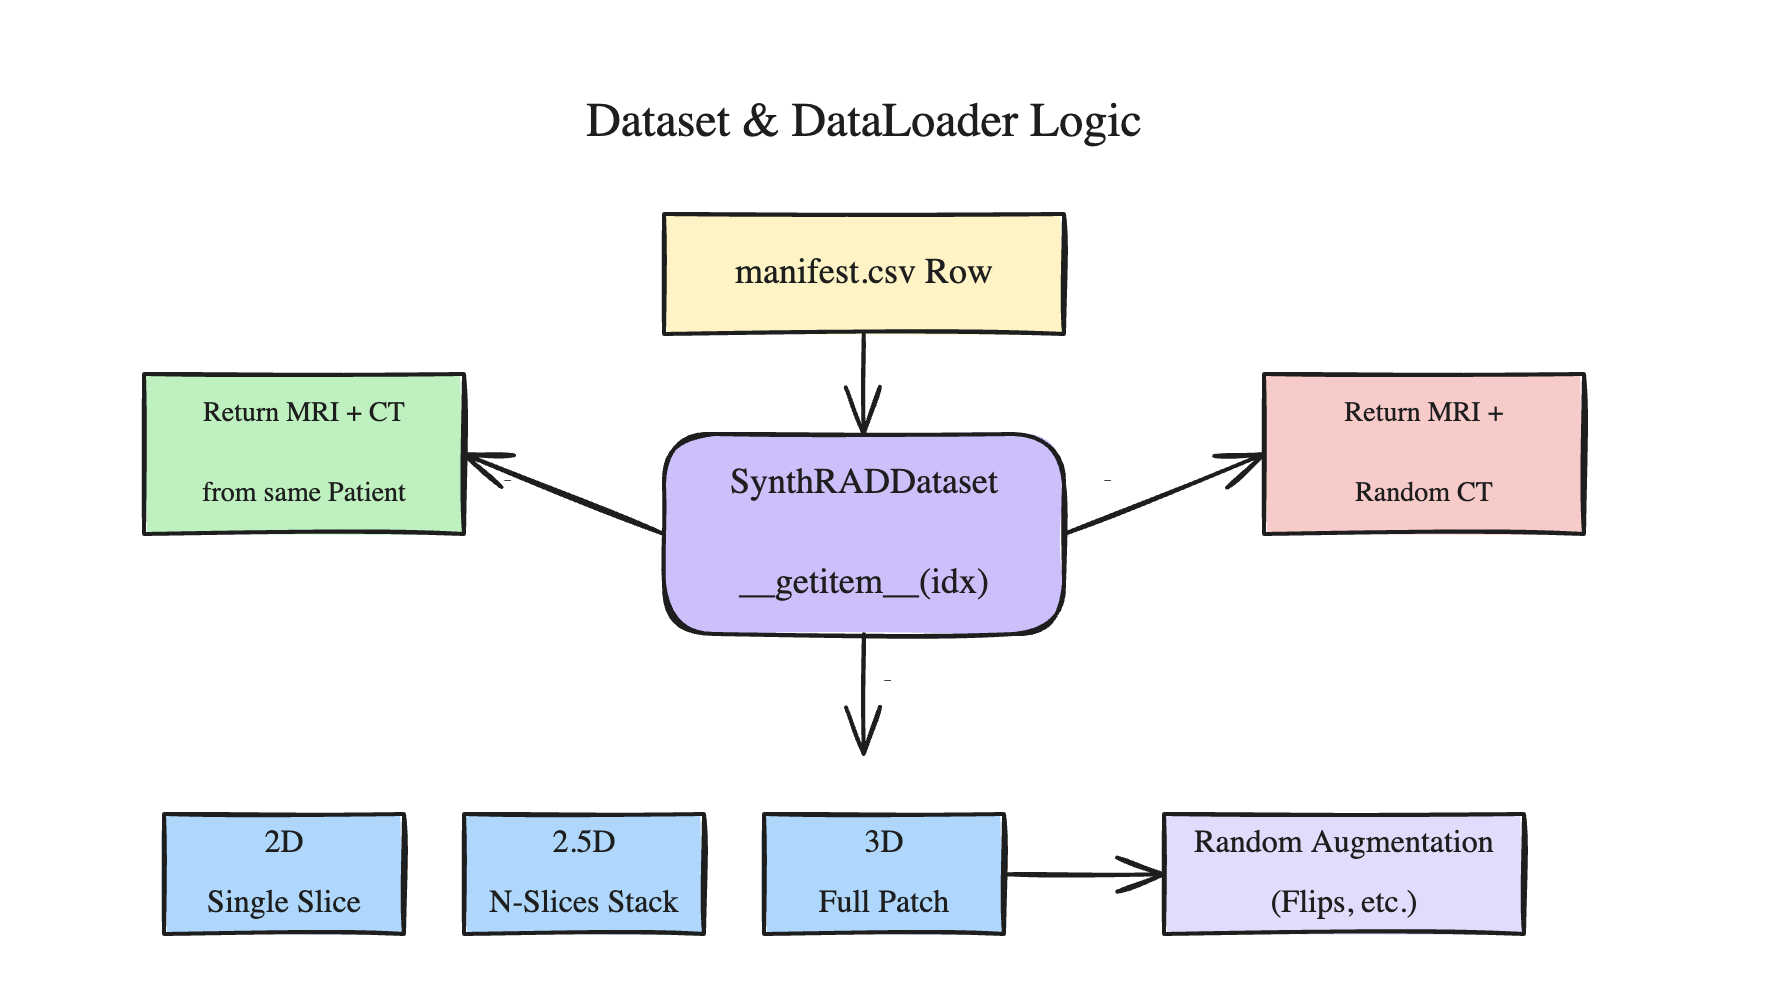
\includegraphics[width=0.92\textwidth]{dataset_and_dataloader_logic.png}
\end{center}
\vspace{-1mm}
\footnotesize
Content-aware slice filter ($\mu_{\text{fg}}>{-}0.9$, $\sigma>0.05$); synced H/V flips for paired pipelines; masked loss zone fixed at the segmentation foreground to suppress background drift.
\end{frame}


% =========================================================================
\section{Model Architectures}
% =========================================================================
\begin{frame}{The 8-Model Factorial Design}
\centering
\footnotesize
\renewcommand{\arraystretch}{1.15}
\begin{tabular}{l|cc|cc}
\toprule
 & \multicolumn{2}{c|}{\textbf{GAN backbone}} & \multicolumn{2}{c}{\textbf{Latent-Diffusion backbone}} \\
\textbf{Pairing} & \textbf{Brain} & \textbf{Pelvis} & \textbf{Brain} & \textbf{Pelvis} \\\midrule
\textbf{Paired}   & Pix2Pix-B  & Pix2Pix-P  & PairedDiff-B  & PairedDiff-P \\
\textbf{Unpaired} & CycleGAN-B & CycleGAN-P & UnpairedDiff-B & UnpairedDiff-P \\
\bottomrule
\end{tabular}
\vspace{2mm}
\begin{block}{Why a fully-crossed design?}
\scriptsize
A balanced $2{\times}2{\times}2$ factorial (\emph{backbone} $\times$ \emph{pairing} $\times$ \emph{region}) lets us decompose the variance into \textbf{main effects} (does pairing help on average?) and an \textbf{interaction} (does pairing help \emph{diffusion} more than GAN?). Identical test-set slices across all four within-region cells enable paired non-parametric tests.
\end{block}
\end{frame}


\begin{frame}{Pix2Pix --- Paired GAN}
\begin{columns}[T]
\begin{column}{0.5\textwidth}
\begin{center}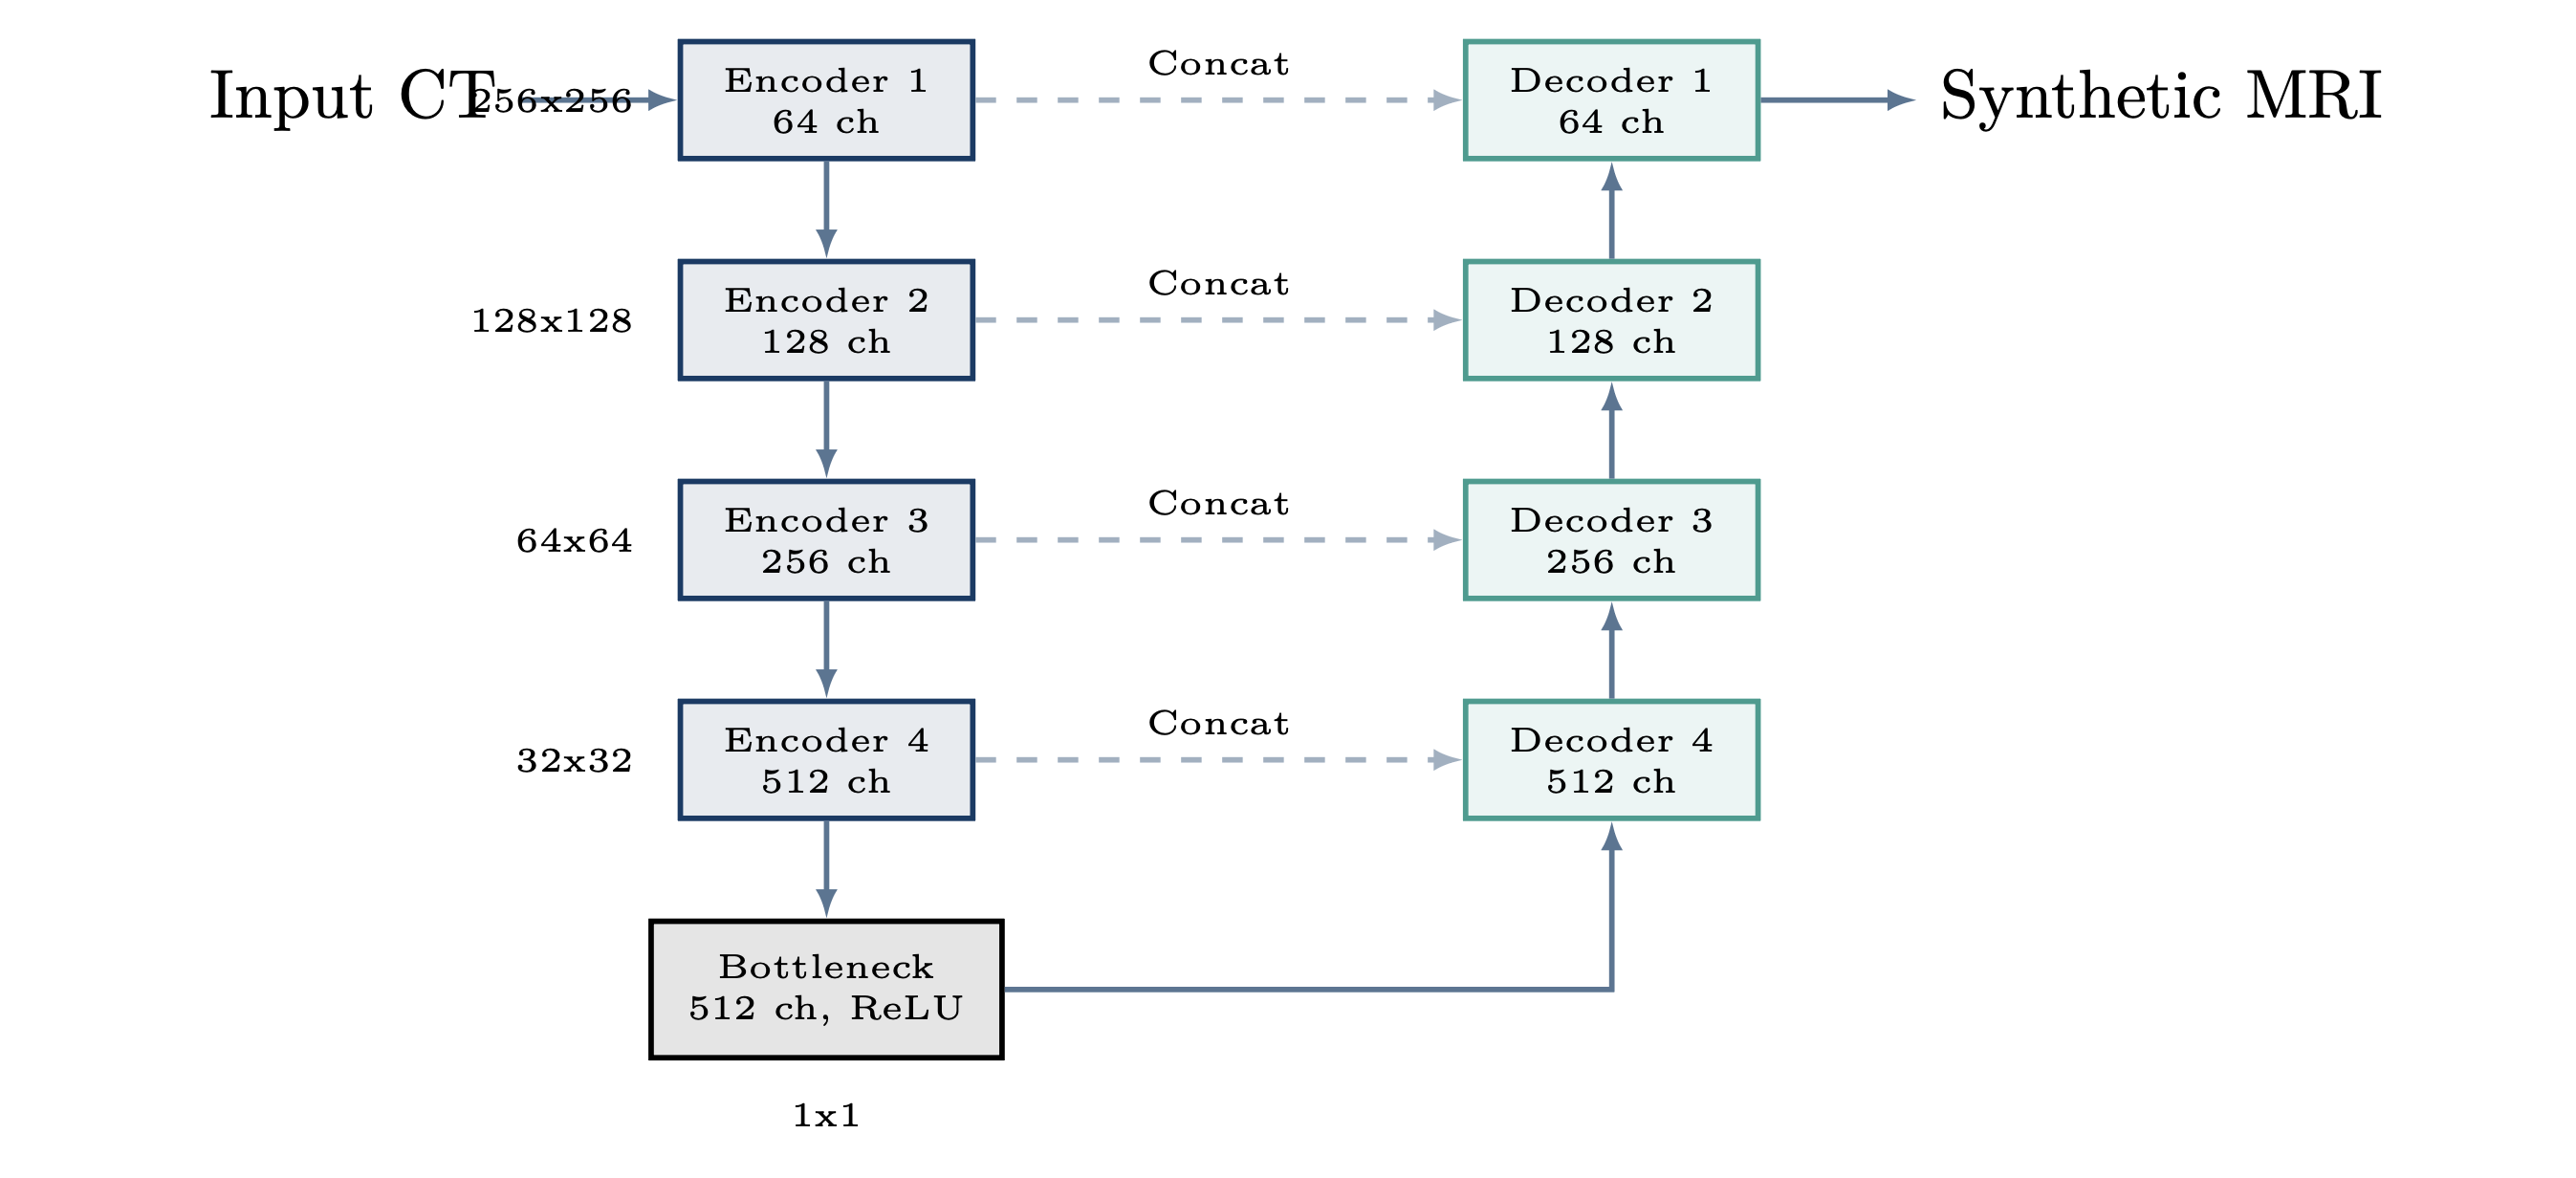
\includegraphics[width=\textwidth]{pix2pix_brain_generator.png}\end{center}
\scriptsize Generator: U-Net (8-layer, skip connections), $4{\times}4$ stride conv, BN, LeakyReLU $\to$ Tanh.
\end{column}
\begin{column}{0.5\textwidth}
\begin{center}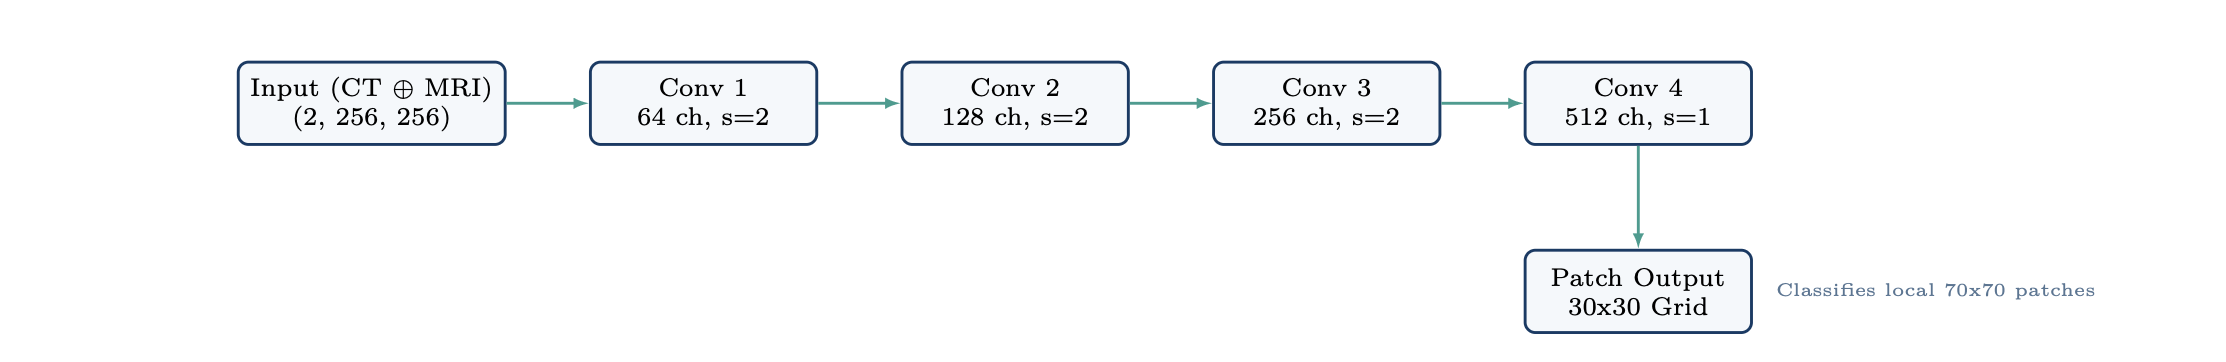
\includegraphics[width=\textwidth]{pix2pix_brain_discriminator.png}\end{center}
\scriptsize Discriminator: $70{\times}70$ PatchGAN on concat$(x,y)$.
\end{column}
\end{columns}
\vspace{1mm}
\footnotesize
\textbf{Loss}\ \  $\mathcal{L}_G = \mathcal{L}_{\text{LSGAN}} + \lambda_{L1}\,\|y-G(x)\|_1$, \ $\lambda_{L1}=100$.\\
Adam ($\beta_1{=}0.5$), LR $2{\times}10^{-4}$, 500 epochs (250 const + 250 decay), batch $1$, BatchNorm.
\end{frame}


\begin{frame}{CycleGAN --- Unpaired GAN}
\begin{columns}[T]
\begin{column}{0.5\textwidth}
\begin{center}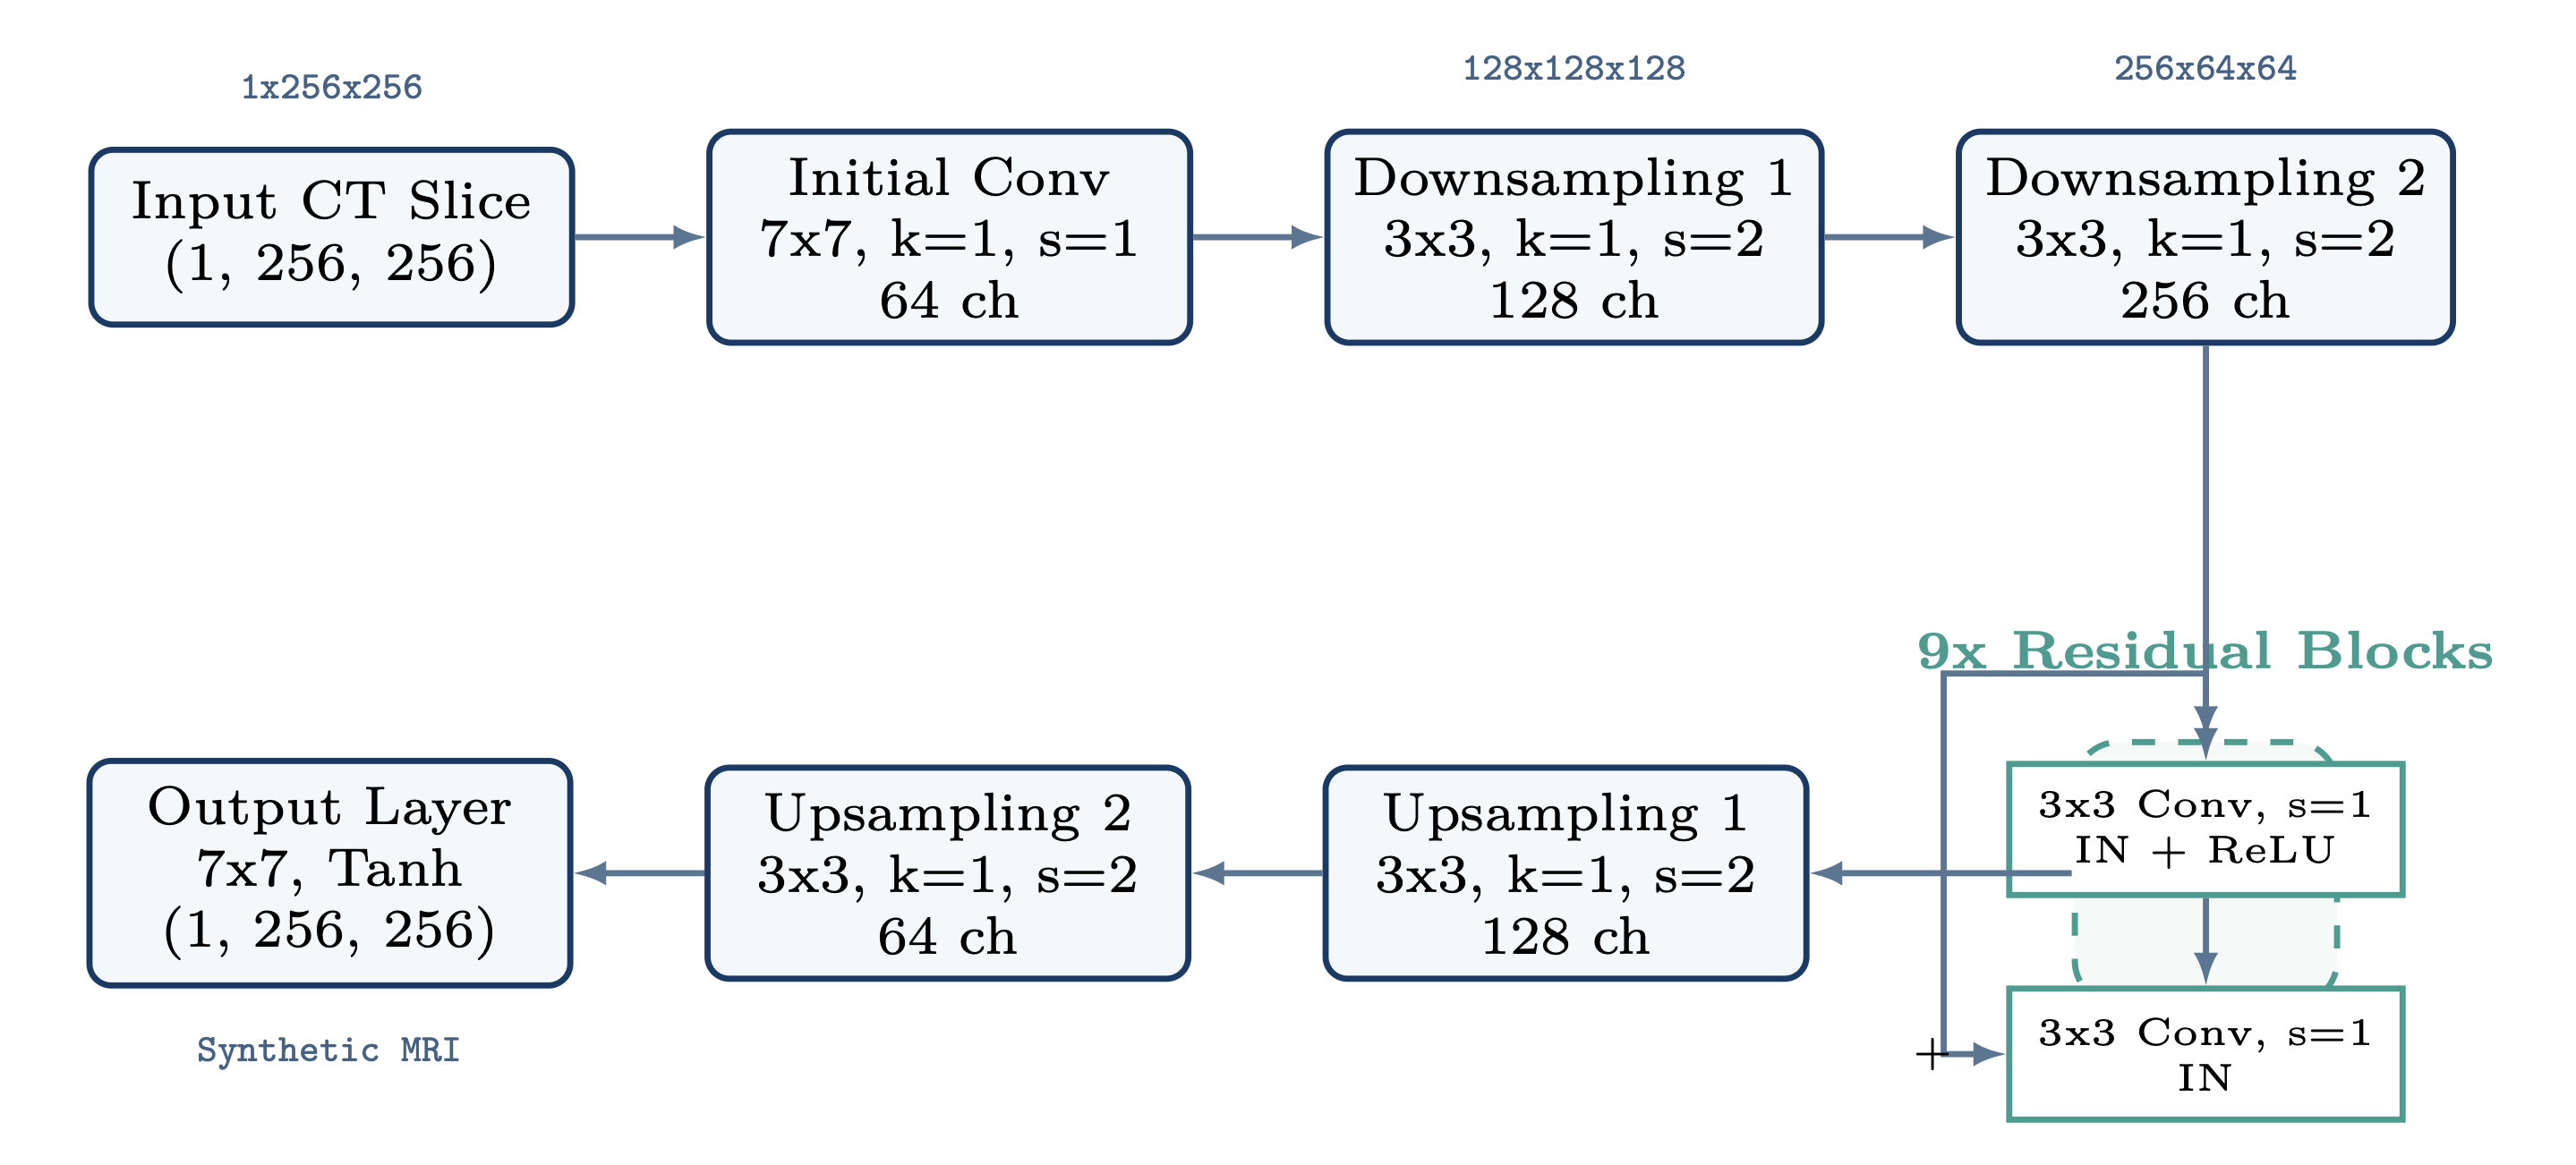
\includegraphics[width=\textwidth]{cyclegan_brain_generator.png}\end{center}
\scriptsize Generator: ResNet-9, $7{\times}7$ reflection-pad, 2$\times$ down/up, optional self-attention.
\end{column}
\begin{column}{0.5\textwidth}
\begin{center}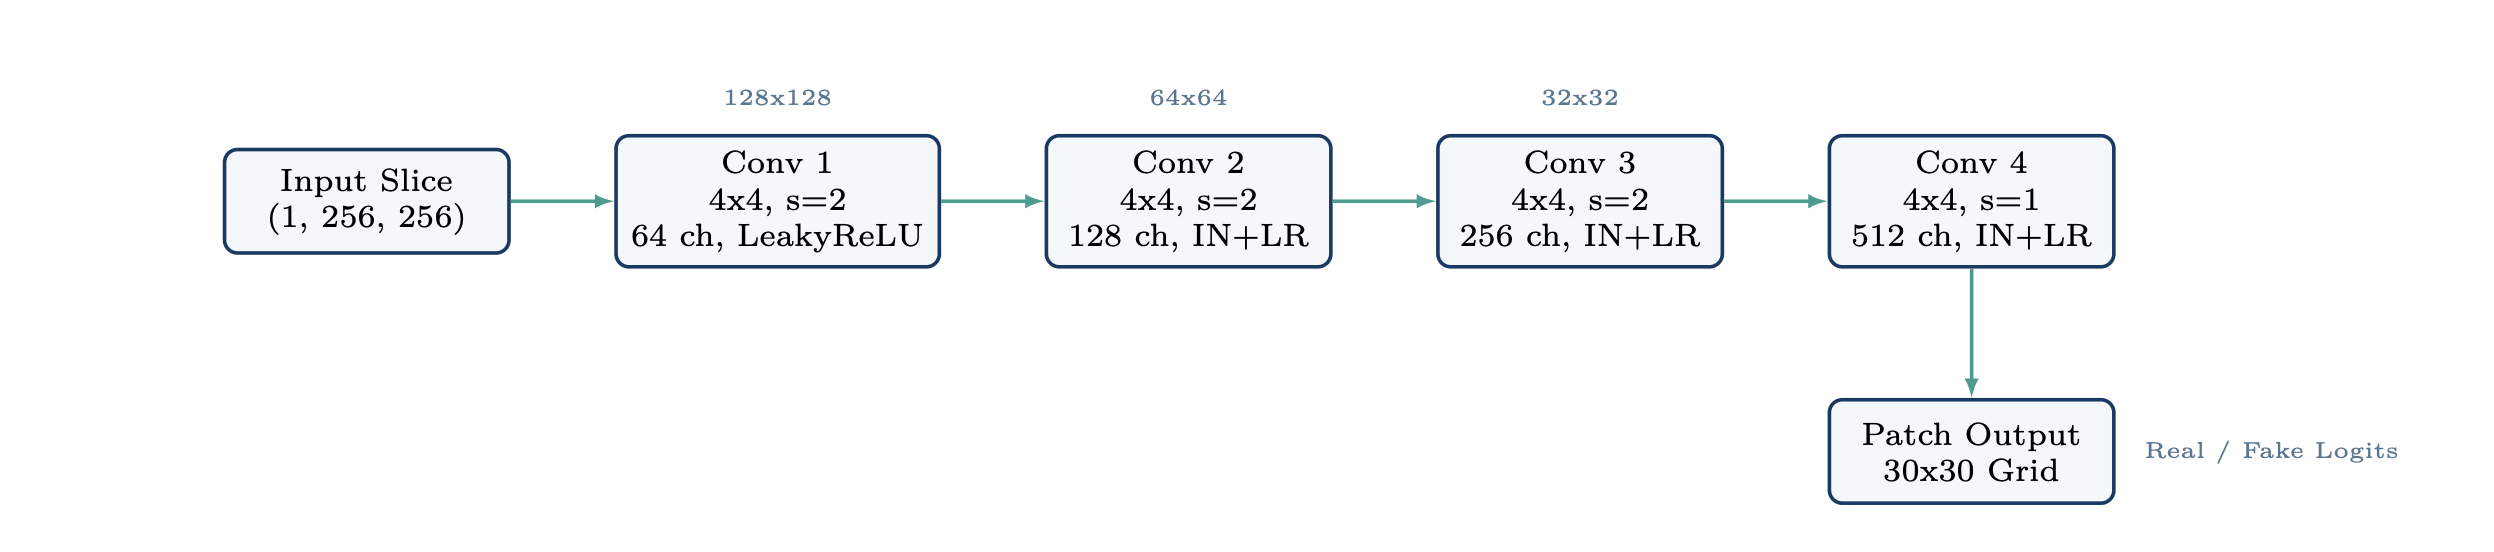
\includegraphics[width=\textwidth]{cyclegan_brain_discriminator.png}\end{center}
\scriptsize Multi-scale PatchGAN (2 scales, $2{\times}$ avg-pool input).
\end{column}
\end{columns}
\vspace{1mm}
\footnotesize
\textbf{Losses}\ \ adversarial $+\;\lambda_{\text{cyc}}\!\cdot\!\mathcal{L}_{\text{cyc}} + \lambda_{\text{idt}}\!\cdot\!\mathcal{L}_{\text{idt}} + \lambda_{\text{LPIPS}}\!\cdot\!\mathcal{L}_{\text{LPIPS}}$, \ \ $\lambda_{\text{cyc}}{=}10,\;\lambda_{\text{idt}}{=}0.5,\;\lambda_{\text{LPIPS}}{=}1$.\\
Adam, LR $2{\times}10^{-4}$, 500 epochs, Instance-Norm.
\end{frame}


\begin{frame}{Paired Latent Diffusion --- SD-Turbo + LoRA}
\begin{columns}[T]
\begin{column}{0.55\textwidth}
\begin{center}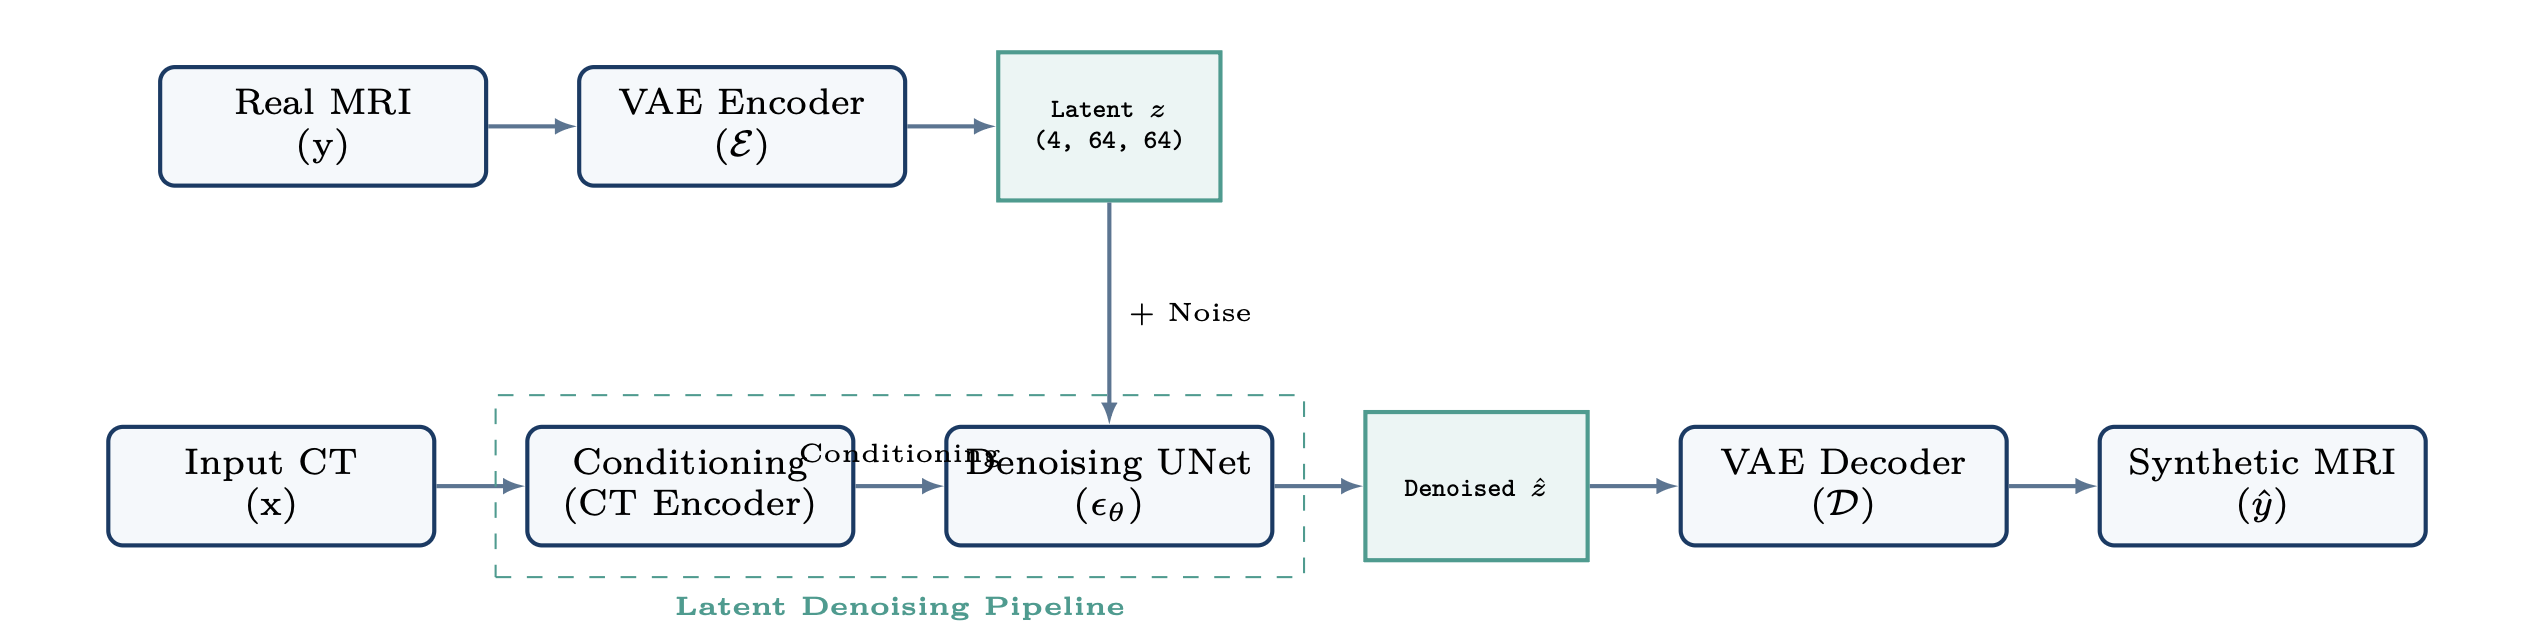
\includegraphics[width=\textwidth]{paired_diffusion_brain.png}\end{center}
\end{column}
\begin{column}{0.42\textwidth}
\begin{block}{Configuration}
\footnotesize
\begin{itemize}
    \item Base: \texttt{stabilityai/sd-turbo} (1-step LDM)
    \item LoRA: UNet rank $r{=}8$, VAE rank $r{=}4$
    \item Resolution $512^{2}$, 2.5D input
    \item AdamW, LR $5{\times}10^{-6}$, grad-accum $8$
\end{itemize}
\end{block}
\begin{block}{Loss}
\scriptsize
$\mathcal{L} = \lambda_{d}\mathcal{L}_{\text{denoise}} + \lambda_{1}\mathcal{L}_{L1} + \lambda_{P}\mathcal{L}_{\text{LPIPS}} + \lambda_{G}\mathcal{L}_{\text{VAGAN-CLIP}}$\\
$\lambda_d{=}1,\,\lambda_1{=}10,\,\lambda_P{=}5,\,\lambda_G{=}0.5$
\end{block}
\end{column}
\end{columns}
\end{frame}


\begin{frame}{Unpaired Cycle-Diffusion --- the focus model}
\begin{columns}[T]
\begin{column}{0.55\textwidth}
\begin{center}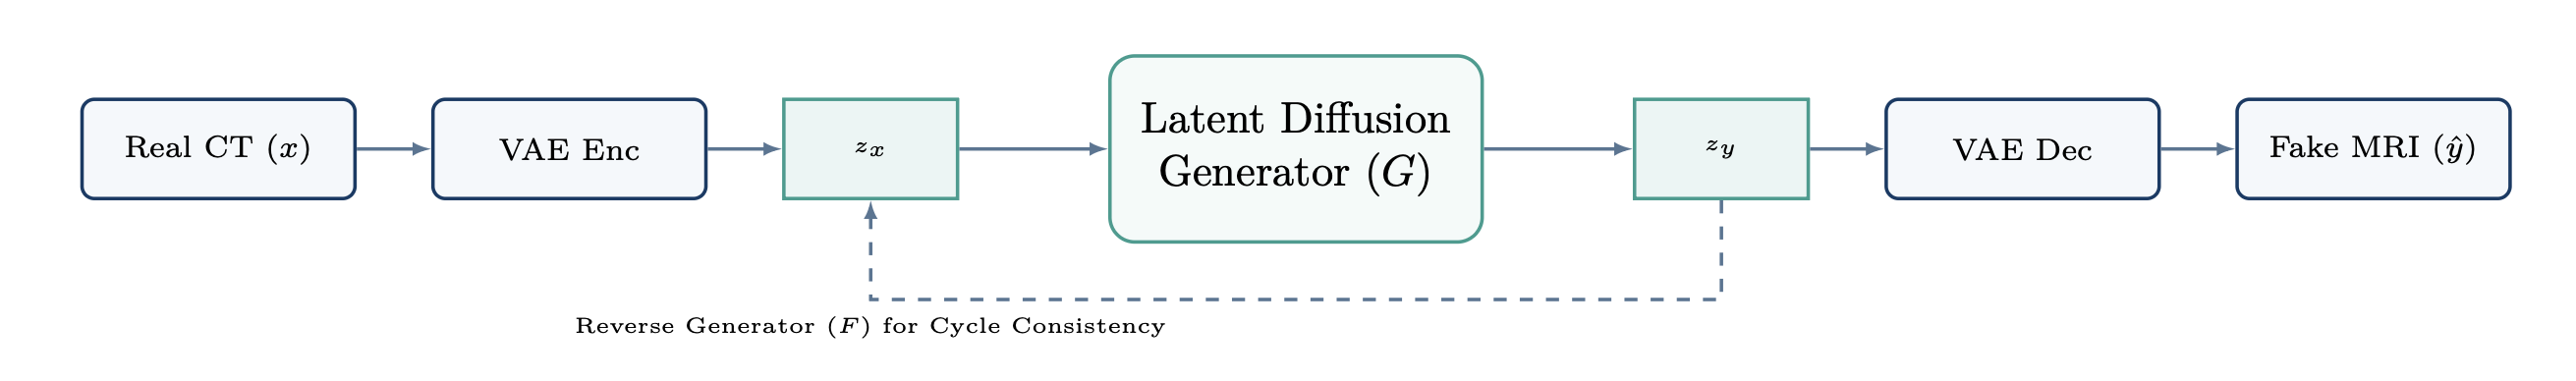
\includegraphics[width=\textwidth]{unpaired_diffusion_brain.png}\end{center}
\end{column}
\begin{column}{0.42\textwidth}
\begin{block}{Why combine cycle + LDM?}
\footnotesize
\begin{itemize}
    \item Cycle gives anatomical \emph{stability} without paired targets
    \item Distilled diffusion prior provides \emph{texture realism}
    \item Dual VAE decoders \texttt{vae\_a2b}, \texttt{vae\_b2a}
\end{itemize}
\end{block}
\begin{block}{Loss}
\scriptsize
$\mathcal{L}_{\text{GAN}} + \lambda_{c}\mathcal{L}_{\text{cyc}} + \lambda_{cp}\mathcal{L}_{\text{cyc-LPIPS}} + \lambda_{i}\mathcal{L}_{\text{idt}} + \lambda_{ip}\mathcal{L}_{\text{idt-LPIPS}}$\\
$\lambda_c{=}1,\,\lambda_{cp}{=}10,\,\lambda_i{=}1,\,\lambda_{ip}{=}1,\,\lambda_{\text{GAN}}{=}0.5$
\end{block}
\end{column}
\end{columns}
\end{frame}


% =========================================================================
\section{Training Setup}
% =========================================================================
\begin{frame}{Why LoRA + 2.5D? --- the practical case}
\begin{columns}[T]
\begin{column}{0.5\textwidth}
\begin{block}{LoRA for medical imaging}
\footnotesize
\begin{tabular}{ll}
\toprule
\textbf{Full FT} & \textbf{LoRA} \\\midrule
$\sim$860\,M params & $<$1\,\% trained \\
80\,GB VRAM & 24\,GB enough \\
Catastrophic forgetting & Preserves prior \\
Days/run & Hours/run \\
\bottomrule
\end{tabular}
\vspace{1mm}\\
With $<$200 paired patients, full fine-tuning is statistically over-parameterised.
\end{block}
\end{column}
\begin{column}{0.48\textwidth}
\begin{block}{2.5D vs 2D vs 3D}
\footnotesize
\begin{itemize}
    \item \textbf{2D}: discards through-plane context, slice flicker
    \item \textbf{3D}: anatomically faithful, but VRAM-prohibitive for SD-Turbo at $512^{2}$
    \item \textbf{2.5D (3-slice)}: best cost/quality trade-off in our setting
\end{itemize}
\end{block}
\begin{exampleblock}{Net effect}
\scriptsize
Diffusion-level perceptual quality at GAN-level training cost --- the practical lever that makes SD-Turbo viable in this regime.
\end{exampleblock}
\end{column}
\end{columns}
\end{frame}


\begin{frame}{Training Configuration --- 8 models}
\centering
\footnotesize
\renewcommand{\arraystretch}{1.1}
\begin{tabular}{lcccc}
\toprule
\textbf{Hyper-parameter} & \textbf{Pix2Pix} & \textbf{CycleGAN} & \textbf{Paired-Diff} & \textbf{Unpaired-Diff} \\\midrule
Resolution                 & $256^{2}$            & $256^{2}$            & $512^{2}$           & $512^{2}$           \\
Batch size                 & 1                    & 4                    & 1                   & 2                   \\
Epochs                     & 500                  & 500                  & 1000 (18\,k iters)  & 1000 (11.5\,k it.)  \\
Optimizer                  & Adam(0.5,0.999)      & Adam(0.5,0.999)      & AdamW(0.9,0.999)    & AdamW(0.9,0.999)    \\
LR ($G$)                   & $2{\times}10^{-4}$   & $2{\times}10^{-4}$   & $5{\times}10^{-6}$  & $5{\times}10^{-6}$  \\
Schedule                   & Linear decay         & Linear decay         & Constant + warmup   & Constant + warmup   \\
Norm                       & BatchNorm            & InstanceNorm         & --                  & --                  \\
Grad. accum.               & 1                    & 1                    & 8                   & 1                   \\
Trained per region         & Brain, Pelvis        & Brain, Pelvis        & Brain, Pelvis       & Brain, Pelvis       \\
\bottomrule
\end{tabular}
\vspace{1mm}
\begin{alertblock}{Hardware}
\scriptsize NVIDIA RTX A6000 (48\,GB). Patient-wise split fixed across all eight runs.
\end{alertblock}
\end{frame}


% =========================================================================
\section{Quantitative Results}
% =========================================================================
\begin{frame}{Test-Set Metrics --- All 8 Models}
\centering
\renewcommand{\arraystretch}{1.05}
\scalebox{0.78}{
\begin{tabular}{ll cc cc cc cc}
\toprule
\textbf{Model} & \textbf{Region} & \textbf{SSIM\,$\uparrow$} & \textbf{MS-SSIM\,$\uparrow$} & \textbf{PSNR\,$\uparrow$} & \textbf{LPIPS\,$\downarrow$} & \textbf{MAE\,$\downarrow$} & \textbf{MSE\,$\downarrow$} & \textbf{DICE\,$\uparrow$} & \textbf{FID\,$\downarrow$} \\\midrule
\rowcolor{softbg}\textbf{Paired-Diff}    & Brain  & \textbf{0.589} & \textbf{0.394} & 7.63  & \textbf{0.373} & 0.587 & 0.413 & 0.623 & 317.1 \\
Unpaired-Diff & Brain  & 0.583 & 0.390 & 6.40  & 0.384 & 0.689 & 0.547 & 0.623 & \textbf{313.3} \\
Pix2Pix       & Brain  & 0.540 & 0.327 & 12.55 & 0.384 & 0.313 & 0.135 & \textbf{0.624} & 345.0 \\
CycleGAN      & Brain  & 0.492 & 0.353 & \textbf{13.54} & 0.452 & \textbf{0.266} & \textbf{0.106} & 0.546 & 316.2 \\\midrule
\rowcolor{softbg}\textbf{Paired-Diff}    & Pelvis & \textbf{0.463} & \textbf{0.253} & 5.89  & \textbf{0.500} & 0.555 & 0.390 & 0.704 & 313.6 \\
Unpaired-Diff & Pelvis & 0.454 & 0.250 & 4.87  & 0.513 & 0.637 & 0.491 & 0.704 & \textbf{308.3} \\
Pix2Pix       & Pelvis & 0.404 & 0.206 & 12.46 & 0.511 & \textbf{0.248} & \textbf{0.086} & \textbf{0.704} & 323.3 \\
CycleGAN      & Pelvis & 0.280 & 0.169 & \textbf{10.83} & 0.583 & 0.293 & 0.123 & 0.678 & 309.5 \\
\bottomrule
\end{tabular}}
\vspace{1mm}
\begin{block}{Headline}
\footnotesize
\textbf{Diffusion} owns the perceptual axis (SSIM, MS-SSIM, LPIPS); \textbf{GAN} owns the pixel-error axis (PSNR, MSE, MAE). \textbf{FID} is uninformative (308--345 across the board on 36-patient test). \textbf{DICE} saturates at the dense-tissue mask.
\end{block}
\end{frame}


\begin{frame}{Metric Bars --- Across Models \& Regions}
\begin{center}
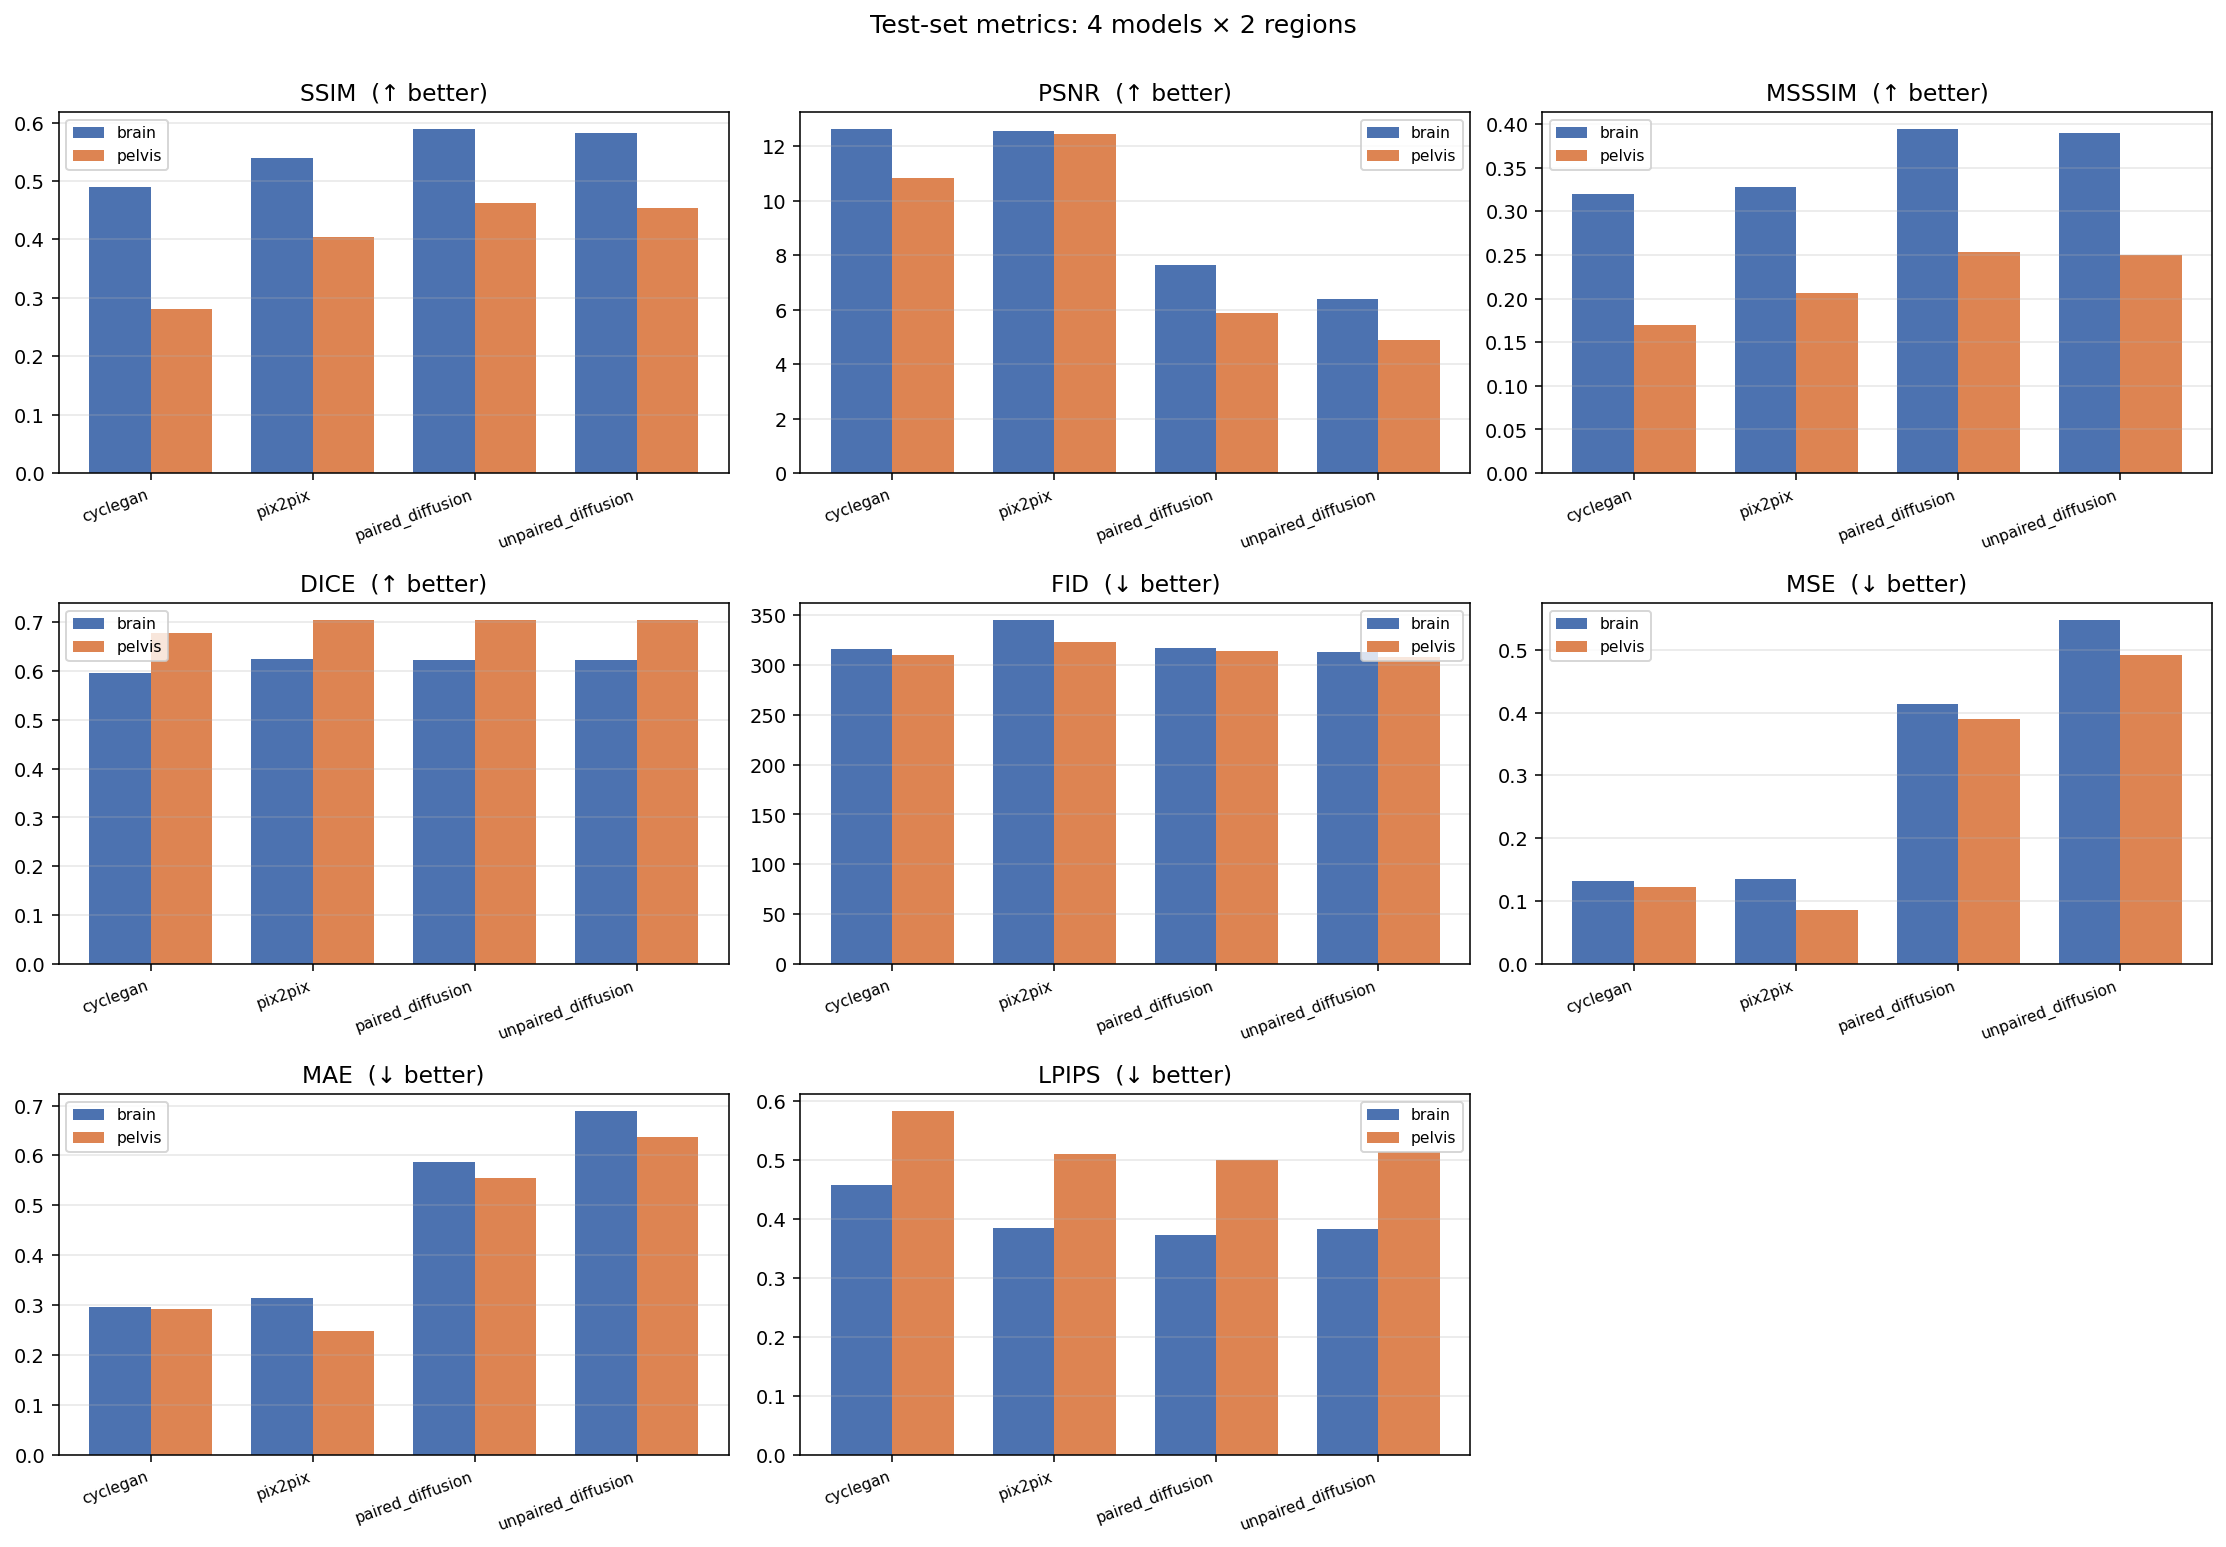
\includegraphics[height=0.78\textheight,keepaspectratio]{metrics_bars.png}
\end{center}
\vspace{-1mm}
\scriptsize
Brain (blue) is uniformly easier than Pelvis (orange). Diffusion sweeps SSIM/MS-SSIM/LPIPS; GANs sweep PSNR/MSE/MAE. Bone-DICE saturates near the mask ratio.
\end{frame}


\begin{frame}{Per-Slice Distributions --- Variance is the story}
\begin{center}
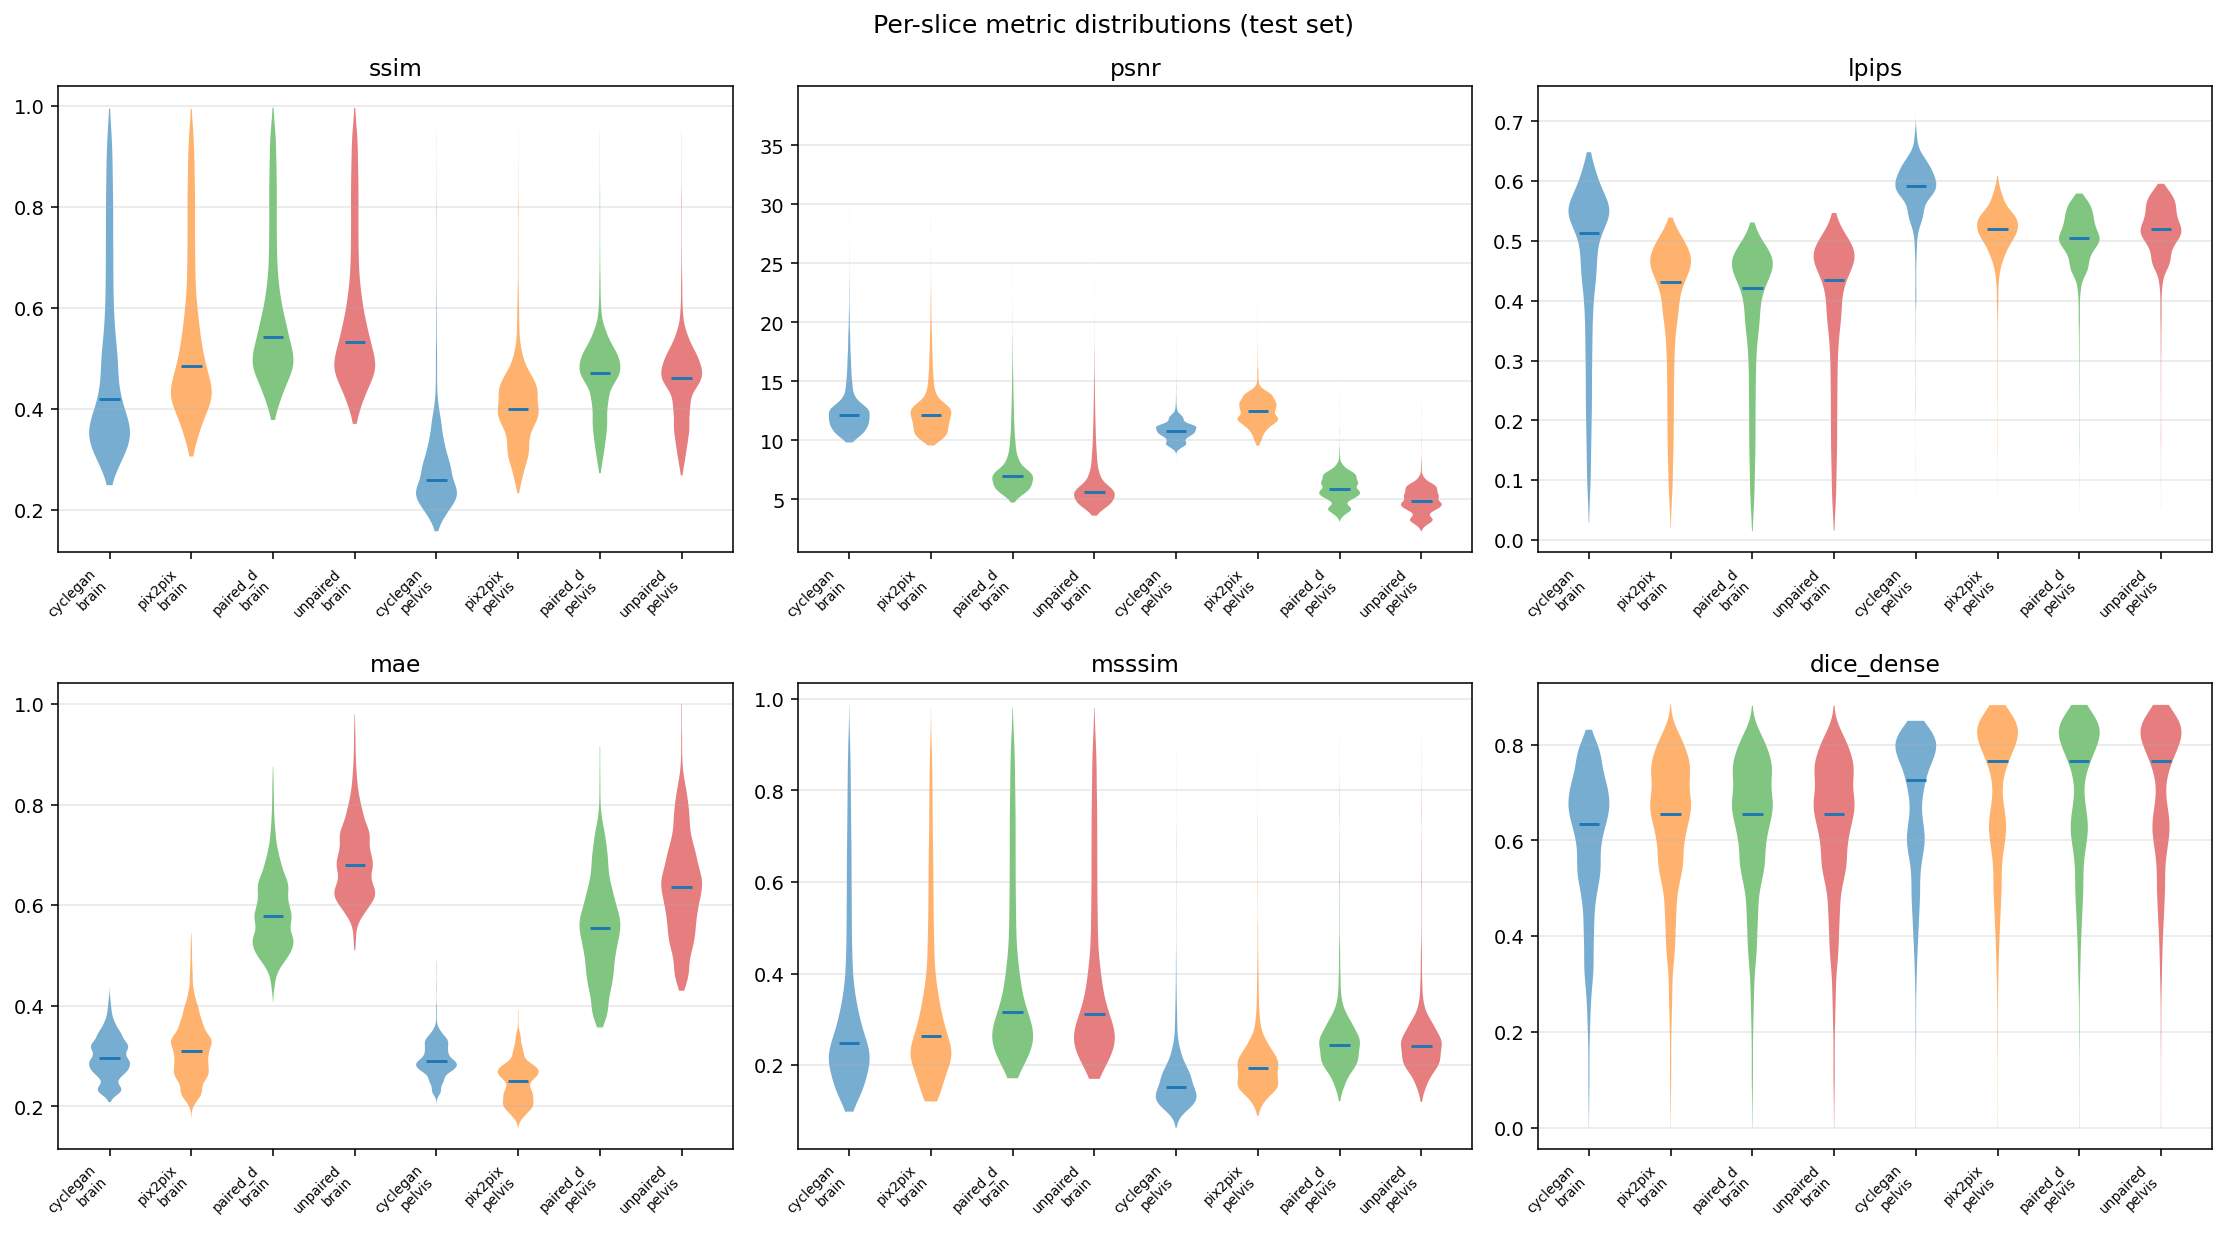
\includegraphics[height=0.78\textheight,keepaspectratio]{metric_violins.png}
\end{center}
\vspace{-3mm}
\footnotesize
Paired-Diff has the \emph{tightest} SSIM tails on brain and the lowest LPIPS dispersion; CycleGAN-Pelvis is the most variable model across every metric.
\end{frame}


% =========================================================================
\section{Training Curves}
% =========================================================================
\begin{frame}{GAN Training Curves --- per-epoch validation}
\begin{center}
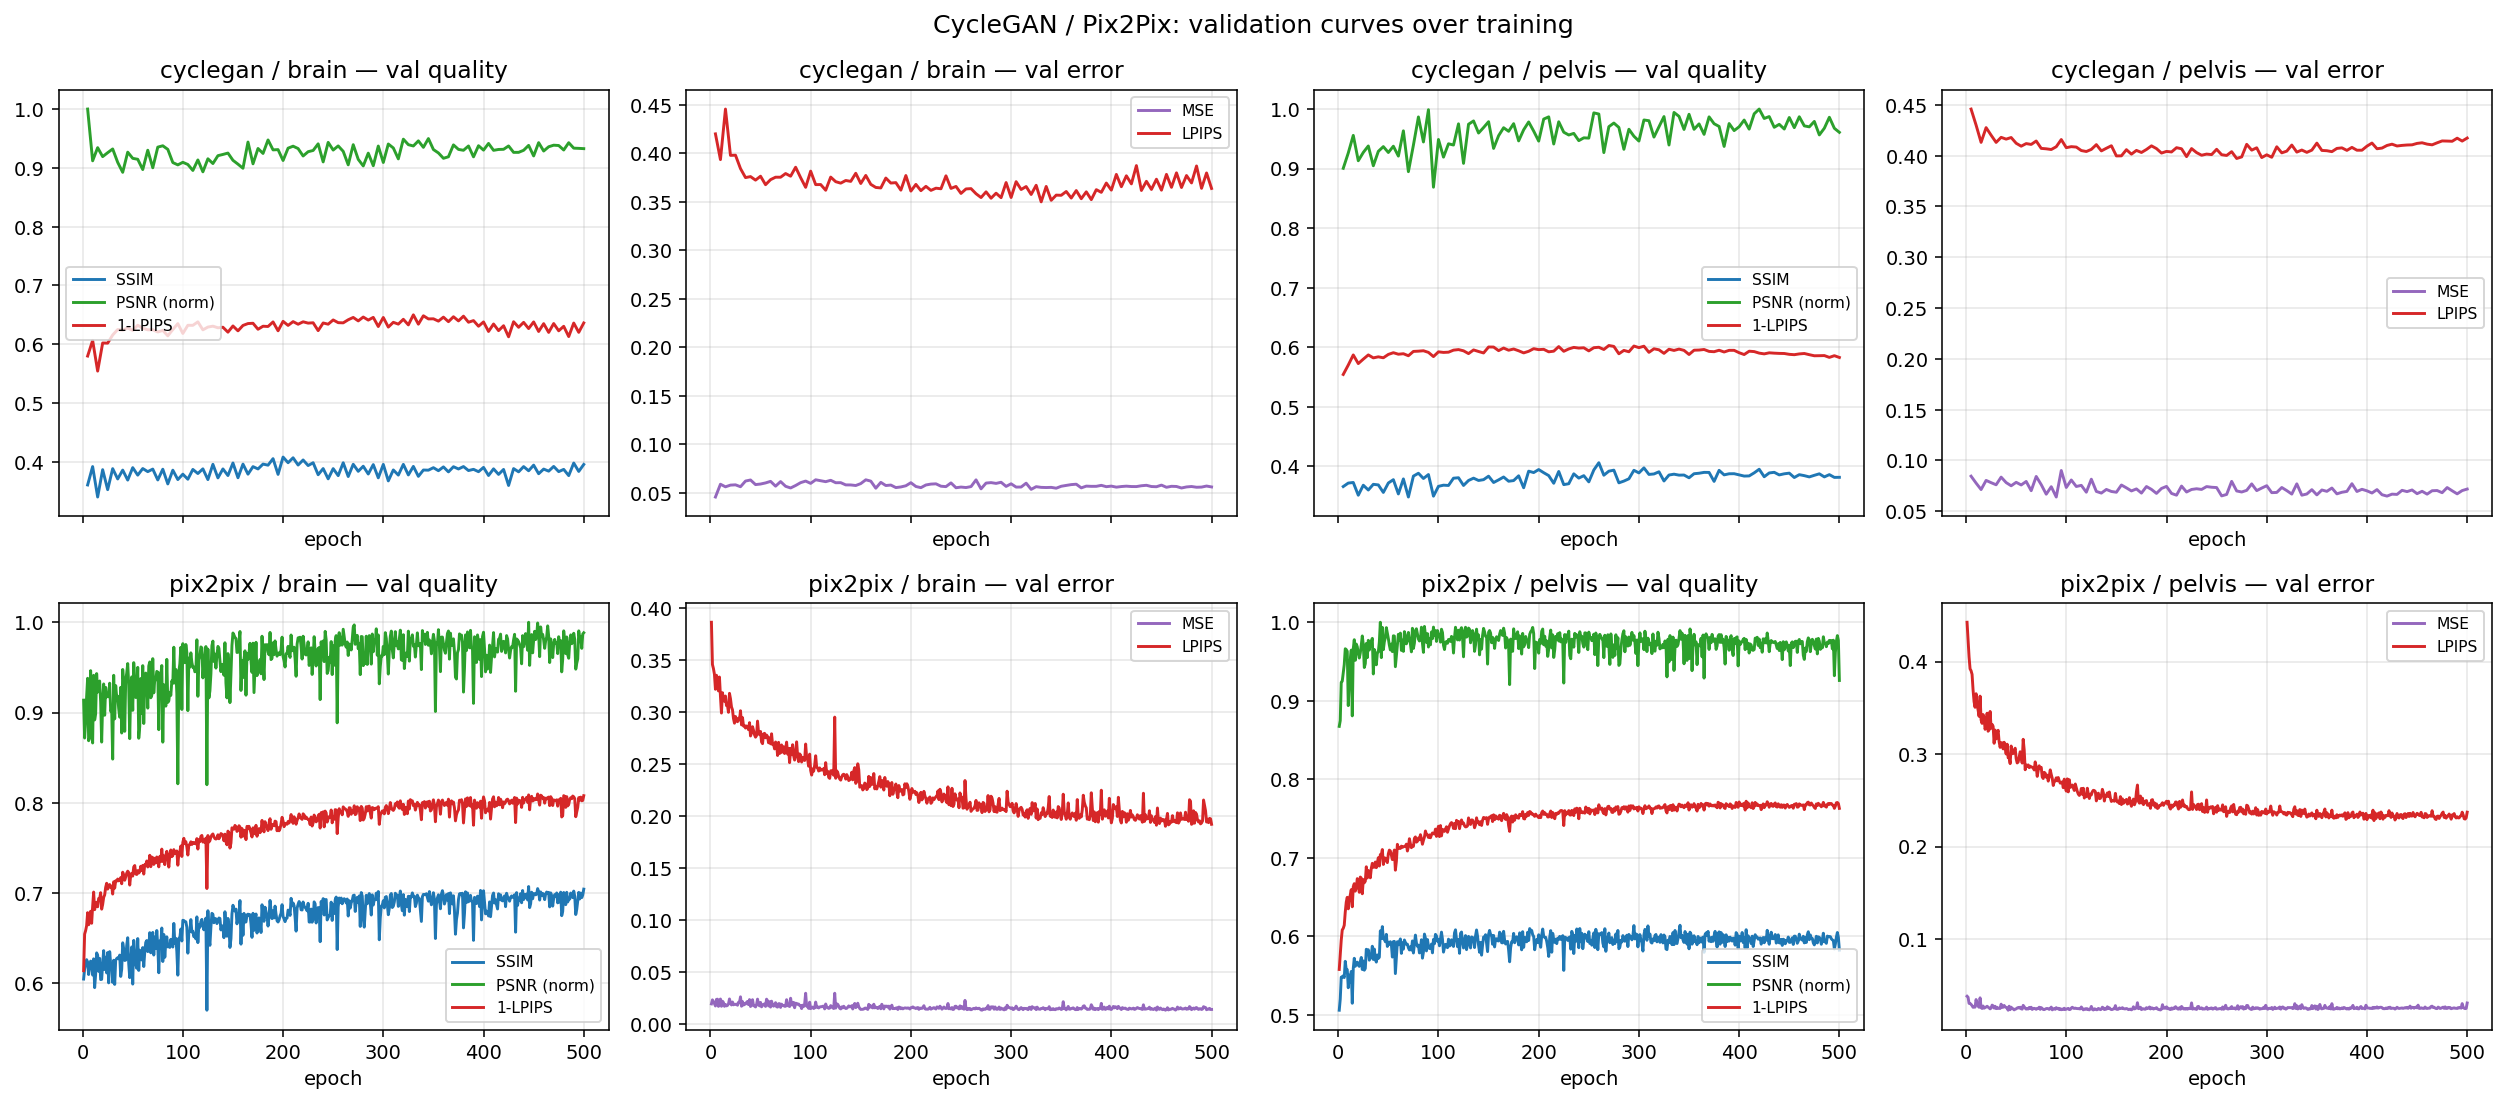
\includegraphics[height=0.78\textheight,keepaspectratio]{gan_training_curves.png}
\end{center}
\vspace{-2mm}
\footnotesize
CycleGAN \& Pix2Pix both reach plateau by epoch ${\sim}300$; Pelvis stays above Brain in LPIPS. Validation MSE stabilises early --- GANs are converged.
\end{frame}


\begin{frame}{Diffusion Training Curves --- per-step losses}
\begin{center}
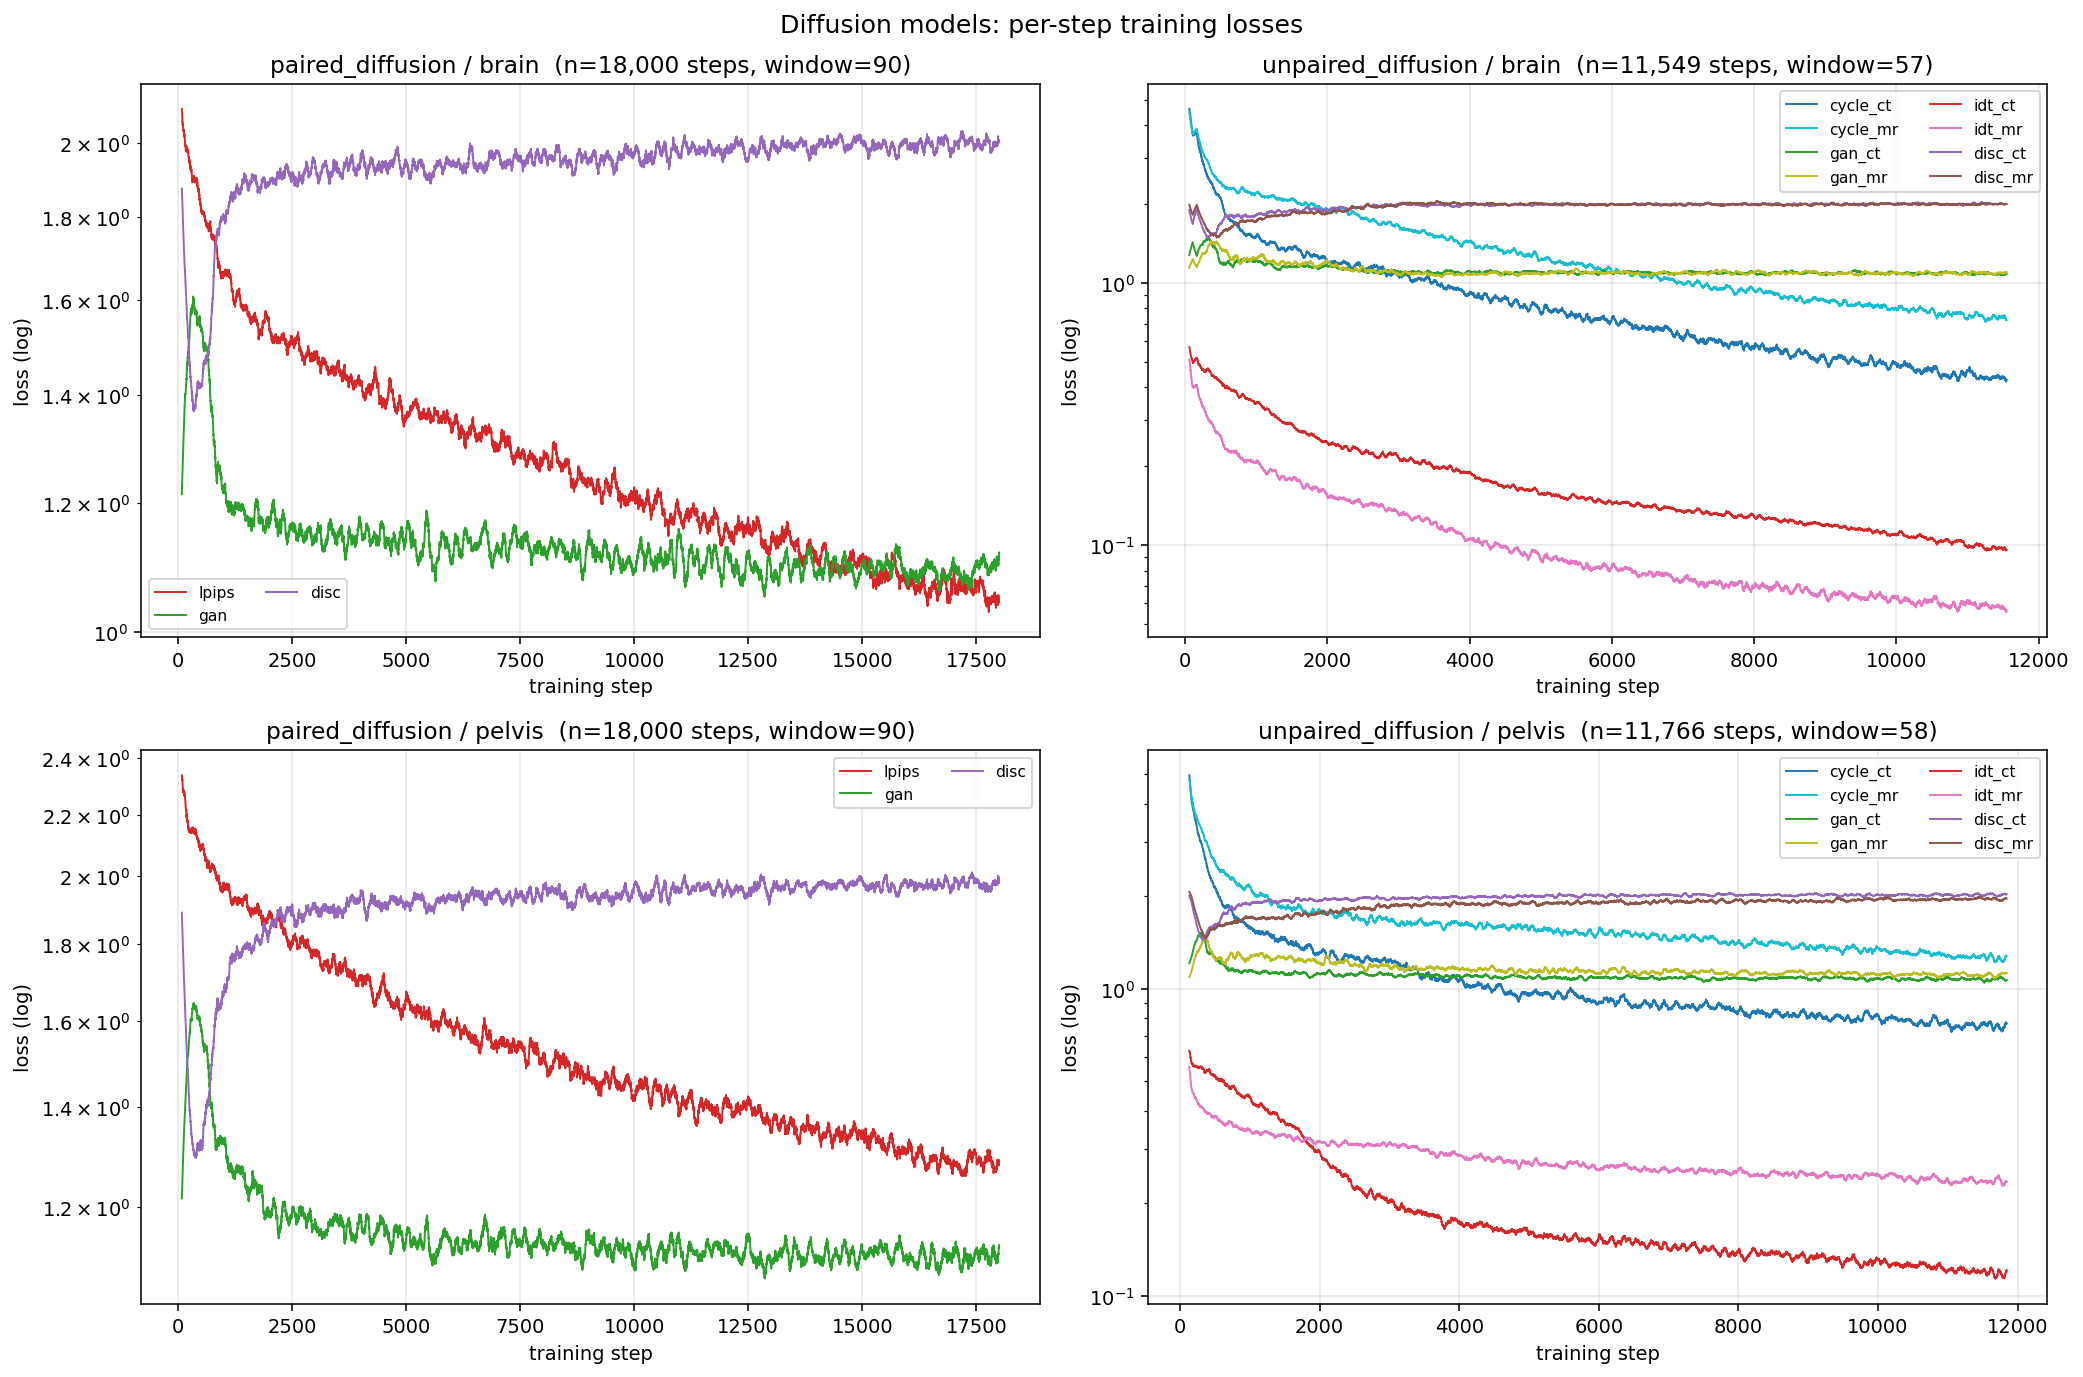
\includegraphics[height=0.78\textheight,keepaspectratio]{diffusion_training_curves.png}
\end{center}
\vspace{-1mm}
\scriptsize
\textbf{Paired-Diff} (left): L1, L2, LPIPS decrease cleanly; GAN/Disc oscillate as expected.\ \ \textbf{Unpaired-Diff} (right): cycle-CT \& cycle-MR converge symmetrically; identity terms and disc are stable, indicating no mode collapse.
\end{frame}


\begin{frame}{LPIPS Across All 8 Models}
\begin{center}
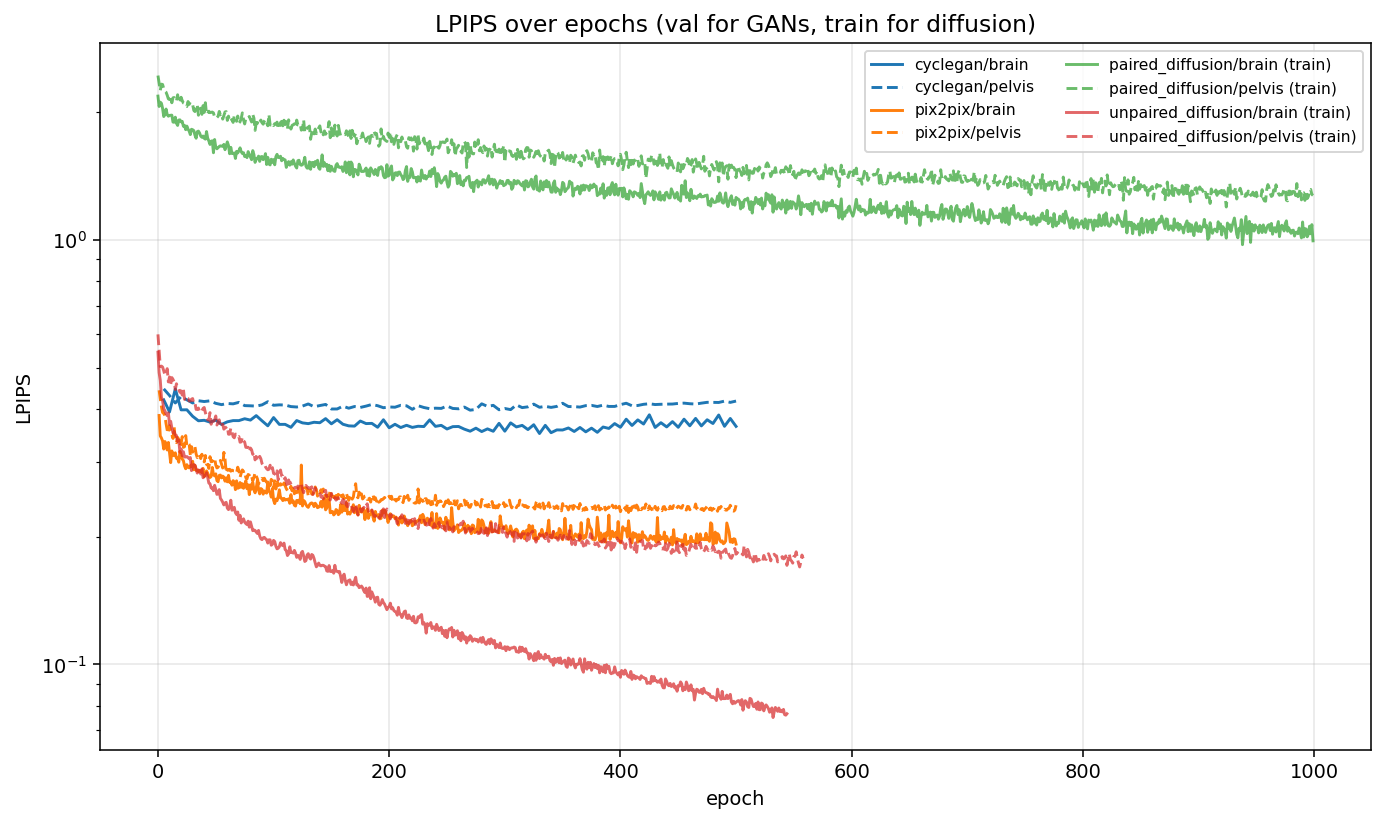
\includegraphics[width=0.78\textwidth]{lpips_overlay.png}
\end{center}
\vspace{-2mm}
\footnotesize
Diffusion variants converge to lower LPIPS than GANs; pelvis lags brain consistently. Both diffusion variants track each other --- the cycle objective costs little perceptually.
\end{frame}


% =========================================================================
\section{Ablation Study}
% =========================================================================
\begin{frame}{Ablation Grid --- Backbone $\times$ Pairing $\times$ Region}
\begin{center}
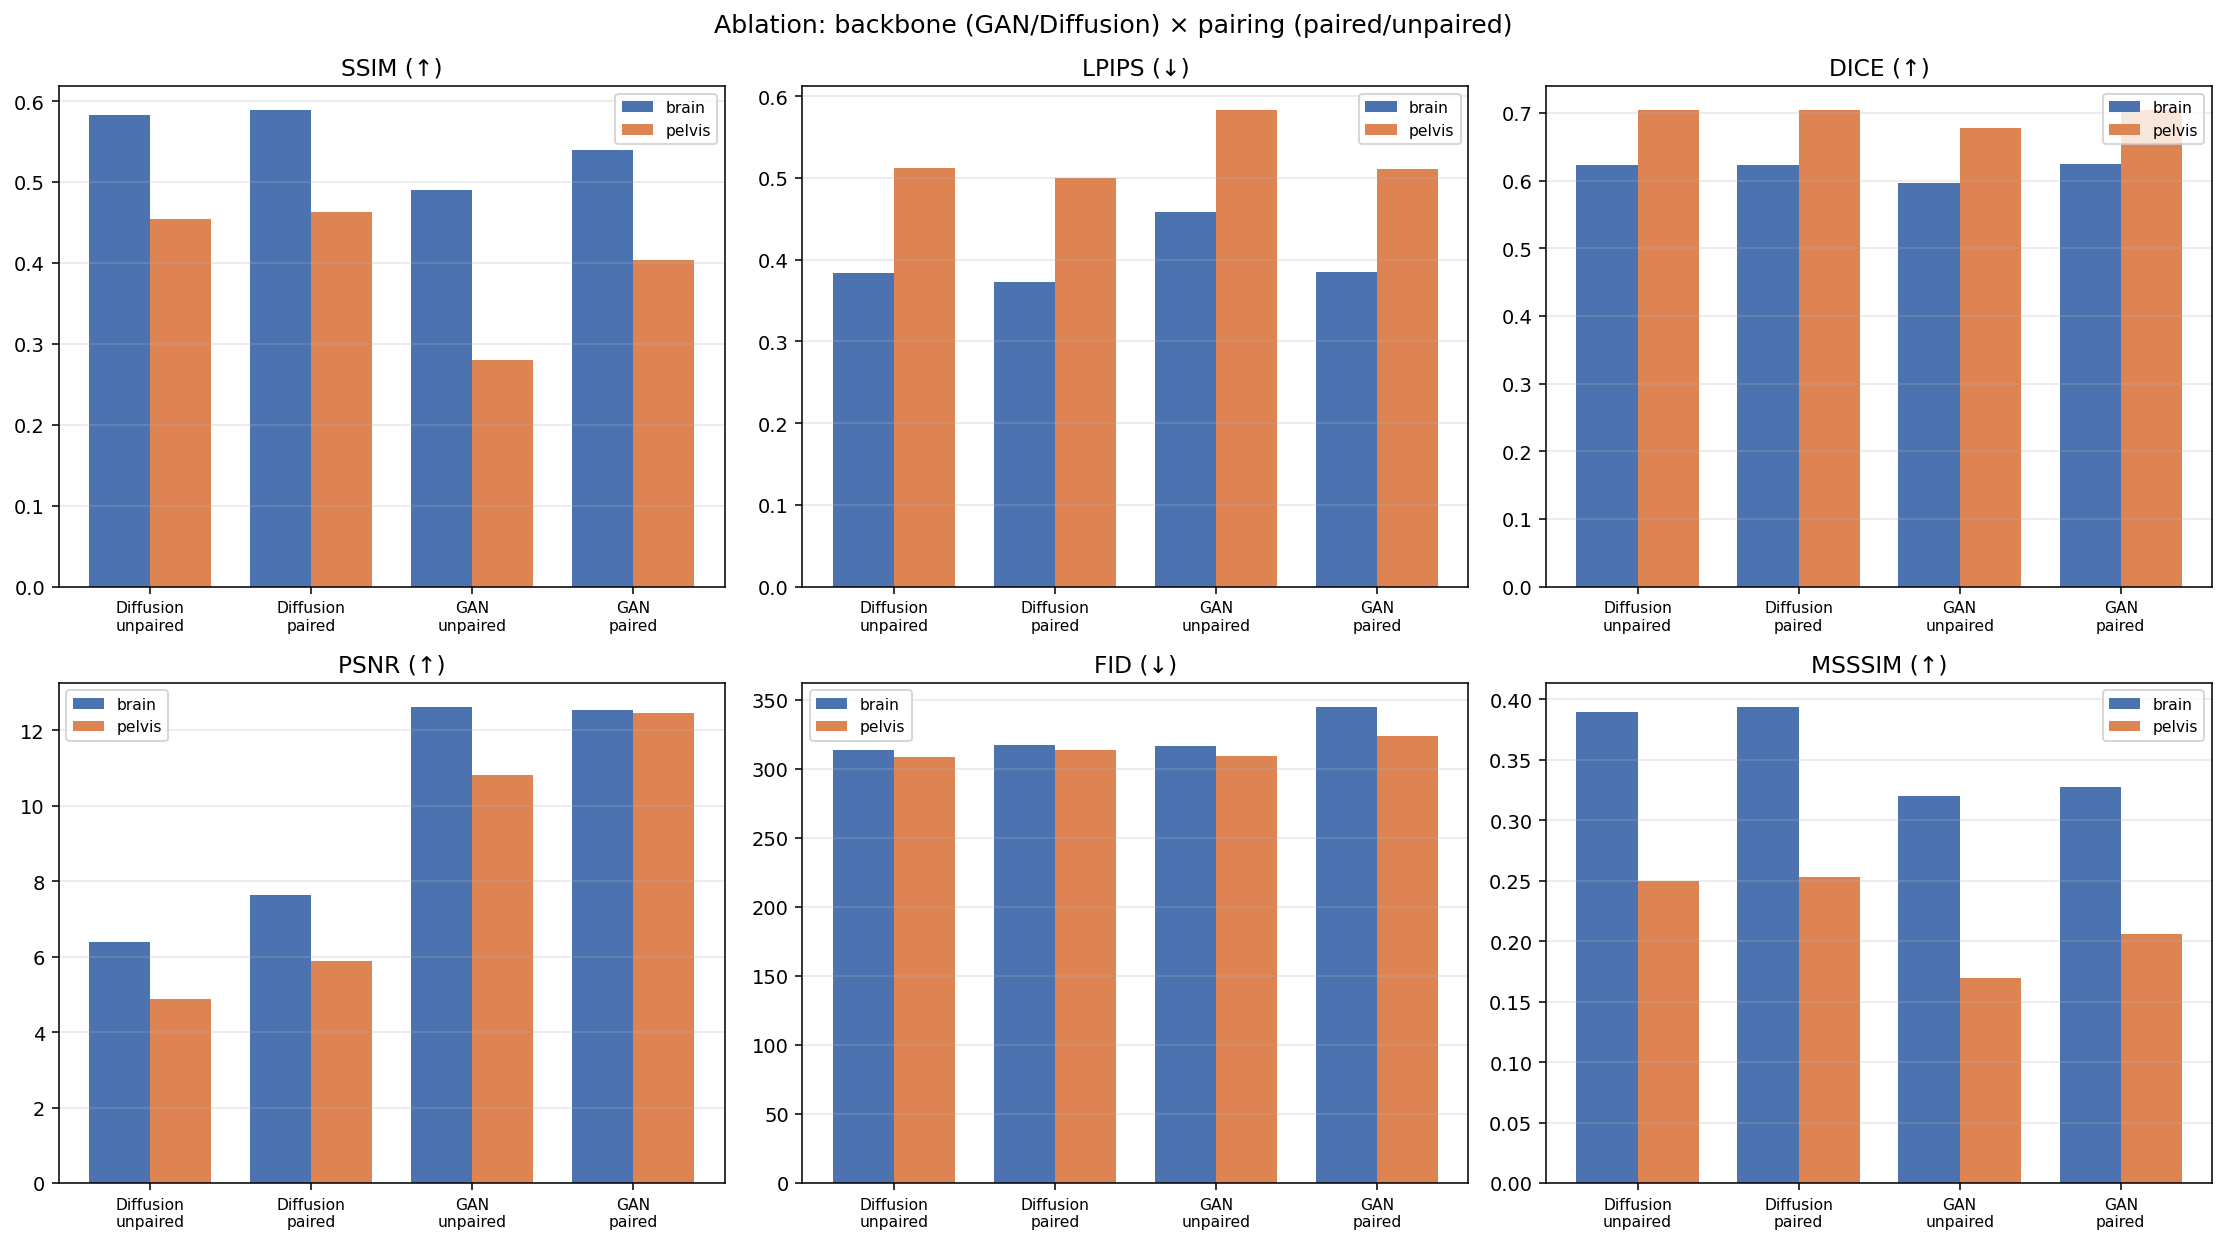
\includegraphics[height=0.78\textheight,keepaspectratio]{ablation_grid.png}
\end{center}
\vspace{-3mm}
\footnotesize
Six key metrics across the four cells of the 2$\times$2 backbone$\times$pairing factorial, separately for brain and pelvis.
\end{frame}


\begin{frame}{Ablation: Statistical Take-aways}
\footnotesize
\begin{block}{(F1) Pairing helps --- consistently}
\begin{itemize}
    \item GAN: pix2pix vs cyclegan SSIM $\Delta\!=\!{+}0.049$ (brain), ${+}0.123$ (pelvis); LPIPS lower.
    \item Diffusion: paired vs unpaired SSIM $\Delta\!=\!{+}0.006$ (brain), ${+}0.008$ (pelvis); MSE/MAE drop ${\sim}0.10$.
\end{itemize}
\end{block}
\begin{block}{(F2) Backbone determines the perceptual$\leftrightarrow$pixel trade-off}
\begin{itemize}
    \item Diffusion sweeps SSIM, MS-SSIM, LPIPS in every region$\times$pairing cell.
    \item GAN sweeps PSNR / MSE / MAE by 5--8\,dB.
\end{itemize}
\end{block}
\begin{block}{(F3) Region effect is large but additive (no interaction)}
\begin{itemize}
    \item Pelvis is uniformly harder (mean SSIM $0.40$ vs brain $0.55$).
    \item Backbone$\times$Pairing interaction $\eta^2\!<\!0.05$ on SSIM \& LPIPS.
\end{itemize}
\end{block}
\begin{block}{(F4) DICE saturates}
\begin{itemize}
    \item Bone/skull mask is recovered well by all four families (DICE $0.55{-}0.71$); finer perceptual differences only show in SSIM/LPIPS.
\end{itemize}
\end{block}
\end{frame}


% =========================================================================
\section{Qualitative Results}
% =========================================================================
\begin{frame}{Qualitative Comparison --- Brain (CT $\to$ MRI, epoch 500)}
\begin{columns}[T]
\begin{column}{0.5\textwidth}
\centering\footnotesize Pix2Pix\\
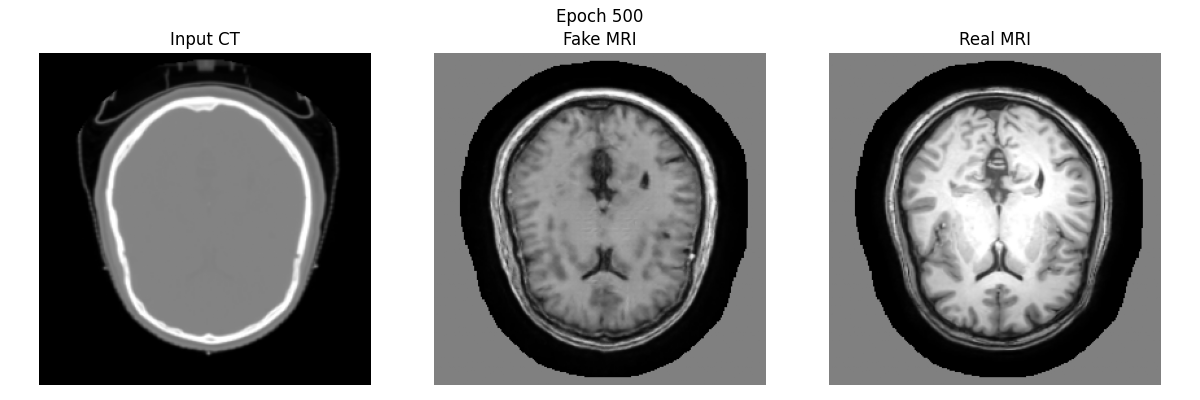
\includegraphics[width=\textwidth]{pix2pix_brain_500.png}
\end{column}
\begin{column}{0.5\textwidth}
\centering\footnotesize CycleGAN\\
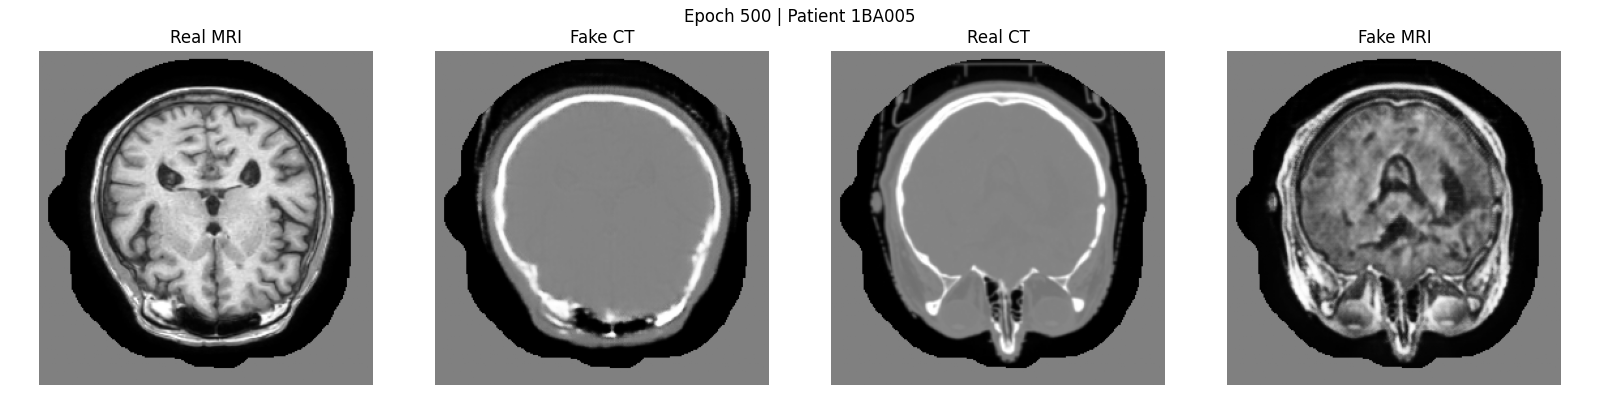
\includegraphics[width=\textwidth]{cyclegan_brain_500.png}
\end{column}
\end{columns}
\vspace{2mm}
\begin{columns}[T]
\begin{column}{0.5\textwidth}
\centering\footnotesize Paired Diffusion\\
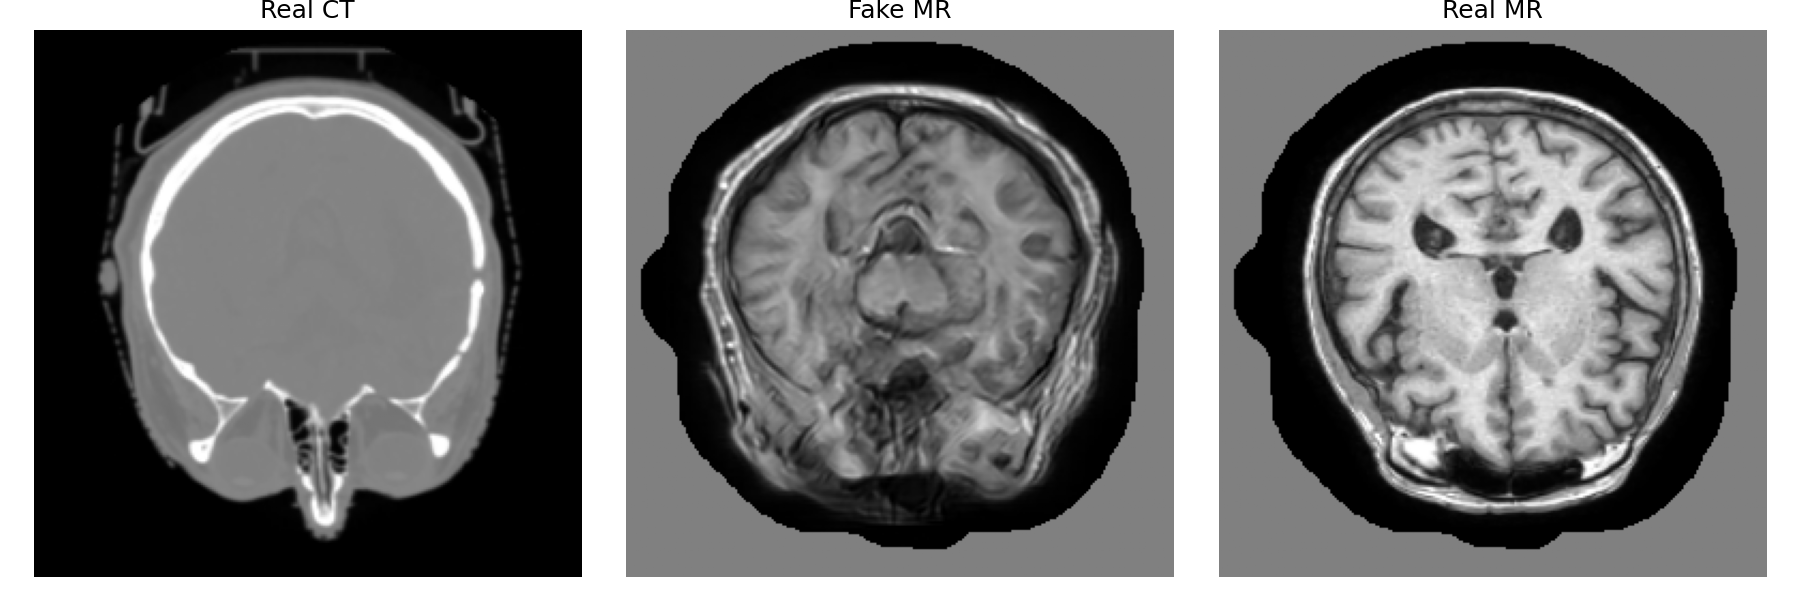
\includegraphics[width=\textwidth]{paired_diff_brain_500.png}
\end{column}
\begin{column}{0.5\textwidth}
\centering\footnotesize Unpaired Cycle-Diffusion\\
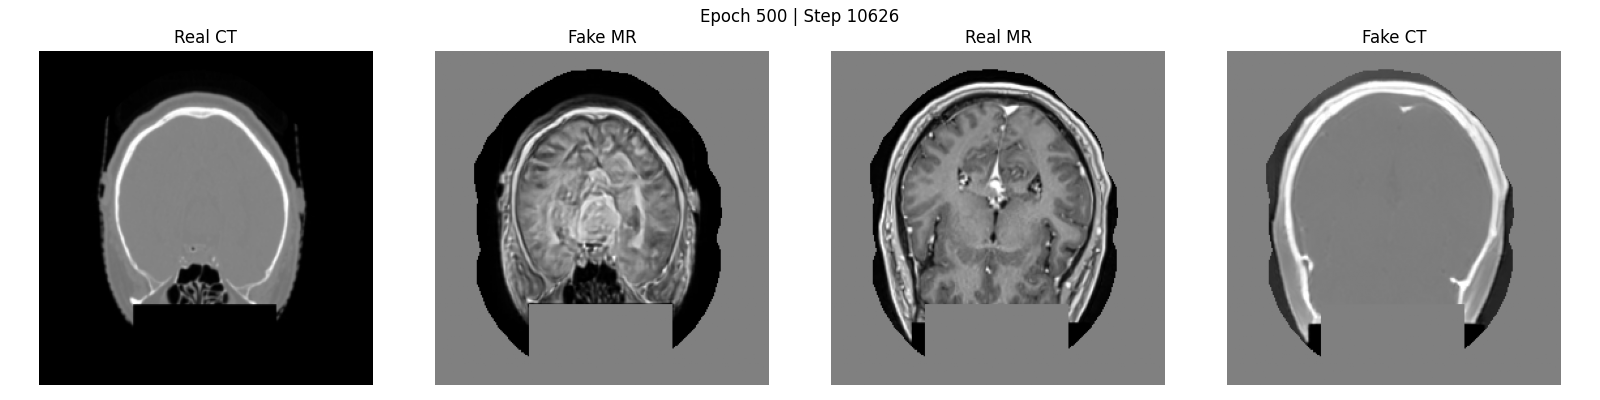
\includegraphics[width=\textwidth]{unpaired_diff_brain_500.png}
\end{column}
\end{columns}
\end{frame}


\begin{frame}{Qualitative Comparison --- Pelvis (CT $\to$ MRI, epoch 500)}
\begin{columns}[T]
\begin{column}{0.5\textwidth}
\centering\footnotesize Pix2Pix\\
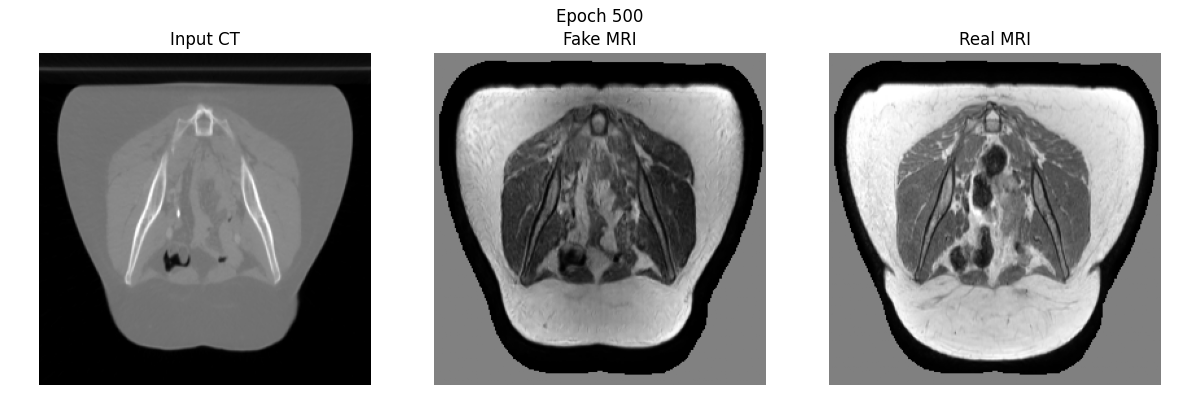
\includegraphics[width=\textwidth]{pix2pix_pelvis_500.png}
\end{column}
\begin{column}{0.5\textwidth}
\centering\footnotesize CycleGAN\\
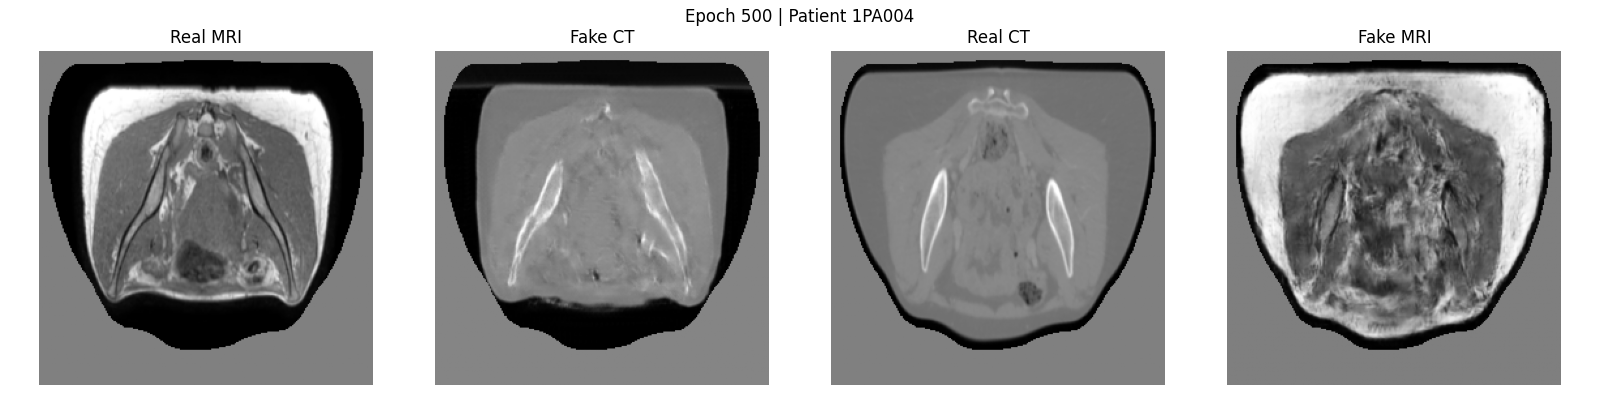
\includegraphics[width=\textwidth]{cyclegan_pelvis_500.png}
\end{column}
\end{columns}
\vspace{2mm}
\begin{columns}[T]
\begin{column}{0.5\textwidth}
\centering\footnotesize Paired Diffusion\\
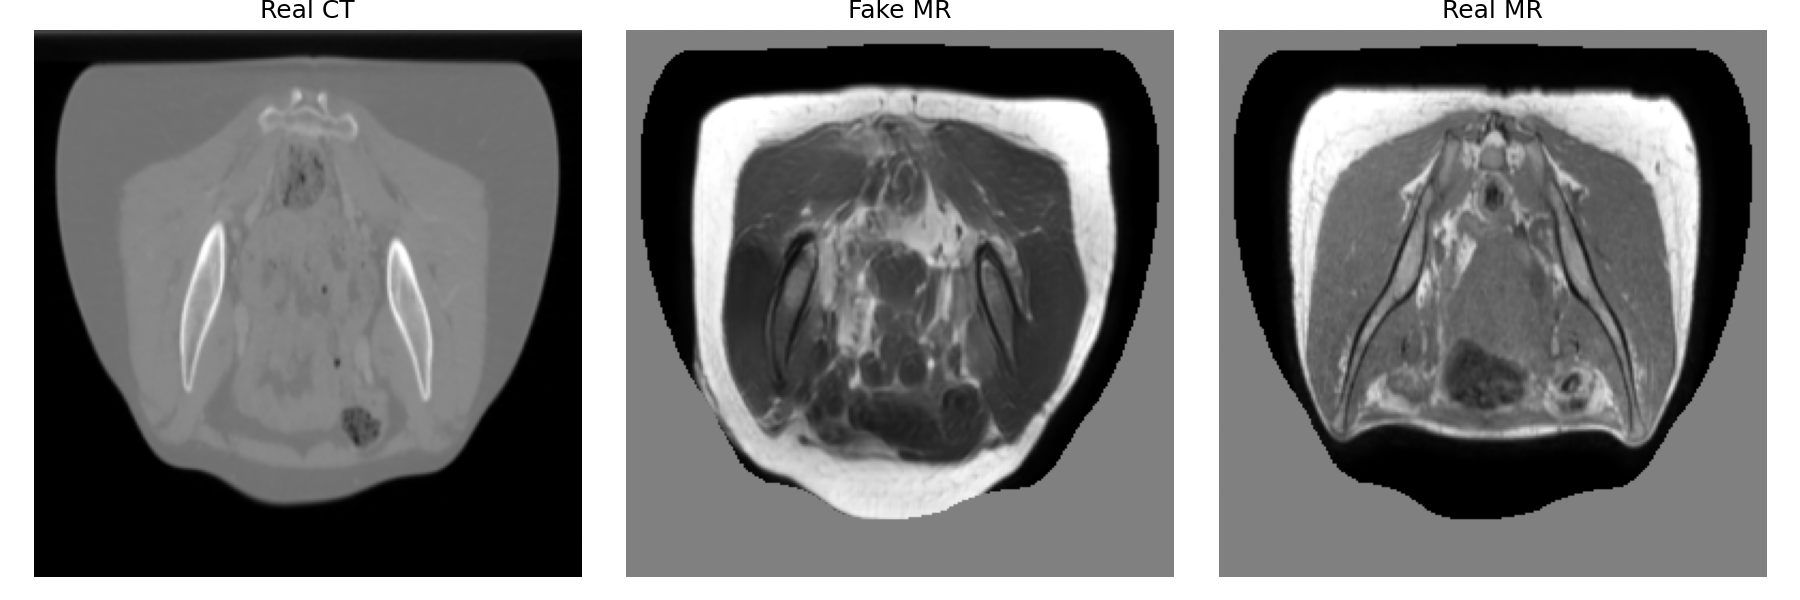
\includegraphics[width=\textwidth]{paired_diff_pelvis_500.png}
\end{column}
\begin{column}{0.5\textwidth}
\centering\footnotesize Unpaired Cycle-Diffusion\\
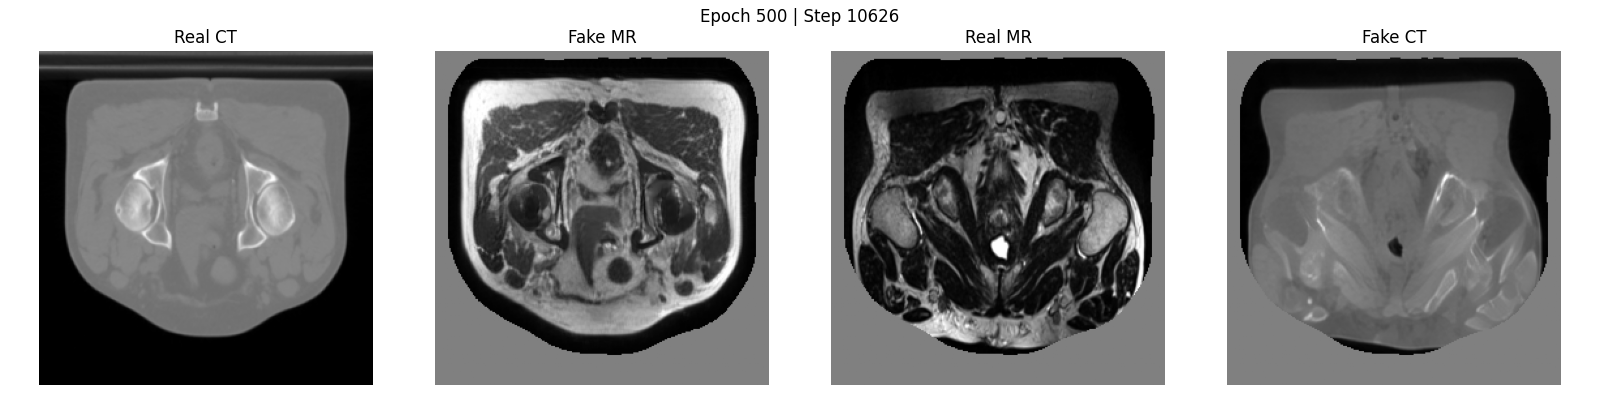
\includegraphics[width=\textwidth]{unpaired_diff_pelvis_500.png}
\end{column}
\end{columns}
\end{frame}


% =========================================================================
\section{Discussion}
% =========================================================================
\begin{frame}{Discussion: the perceptual$\leftrightarrow$pixel split}
\begin{columns}[T]
\begin{column}{0.5\textwidth}
\begin{block}{Interpretation}
\footnotesize
\begin{itemize}
    \item GAN backbones with $L_1$ supervision \textbf{fit the mean intensity} and so dominate PSNR/MAE.
    \item Diffusion backbones generate \textbf{plausible textures} from a learned prior, paying pixel error to gain perceptual similarity.
    \item Under \emph{imperfect pairing}, the perceptual axis is the more clinically relevant one --- a high-PSNR over-smoothed image is not necessarily a more useful image.
\end{itemize}
\end{block}
\end{column}
\begin{column}{0.5\textwidth}
\begin{exampleblock}{Recommendation by use-case}
\footnotesize
\begin{itemize}
    \item \textbf{MR-only RT planning} (downstream dose calc.) $\rightarrow$ \textbf{Pix2Pix}: PSNR/MAE drive dose accuracy.
    \item \textbf{Reader-facing synthetic MRI} or \textbf{soft-tissue review} $\rightarrow$ \textbf{Paired-Diff}: best SSIM/LPIPS.
    \item \textbf{Site with no paired archive} $\rightarrow$ \textbf{Unpaired-Diff}: matches paired diffusion at marginal cost.
    \item \textbf{CycleGAN}: still useful for fast Pelvis bone-mask recovery (DICE $0.68$).
\end{itemize}
\end{exampleblock}
\end{column}
\end{columns}
\end{frame}


\begin{frame}{Limitations \& Honest Discussion}
\footnotesize
\begin{columns}[T]
\begin{column}{0.5\textwidth}
\begin{alertblock}{What we did \emph{not} solve}
\begin{itemize}
    \item \textbf{Volumetric coherence}: results are 2.5D slice-wise; we did not measure inter-slice consistency.
    \item \textbf{Hallucination risk}: cycle losses can paper over anatomy mismatch --- not formally audited per-lesion.
    \item \textbf{FID is weak} on a 36-patient set; cannot rank by it.
    \item \textbf{Single base model}: only SD-Turbo evaluated; SDXL/MedSAM priors untried.
\end{itemize}
\end{alertblock}
\end{column}
\begin{column}{0.5\textwidth}
\begin{block}{What we did do right}
\begin{itemize}
    \item Patient-wise splits (no leakage)
    \item Identical test slices across all 4 models per region $\Rightarrow$ paired Wilcoxon valid
    \item Bootstrap CIs and ANOVA-style ablation
    \item Reported every metric, including ones where we lose
\end{itemize}
\end{block}
\begin{block}{Pix2Pix as upper-bound, not as target}
\scriptsize
Pix2Pix is the \emph{ideal-pairing} ceiling. Our goal is robust performance under \emph{imperfect} pairing --- where Paired-Diff and Unpaired-Diff close the gap on the perceptual axis.
\end{block}
\end{column}
\end{columns}
\end{frame}


% =========================================================================
\section{Conclusion}
% =========================================================================
\begin{frame}{Conclusion \& Future Work}
\begin{columns}[T]
\begin{column}{0.5\textwidth}
\begin{block}{Key findings}
\footnotesize
\begin{enumerate}
    \item 8 models, fully-crossed factorial, patient-wise evaluation.
    \item \textbf{Pairing supervision} yields large, statistically-significant gains in \emph{both} backbones.
    \item \textbf{Backbone} dictates a sharp \textbf{perceptual$\leftrightarrow$pixel} trade-off (Diffusion vs GAN).
    \item \textbf{Region} effect is additive --- no Backbone$\times$Pairing interaction.
    \item LoRA-tuned SD-Turbo achieves diffusion-quality outputs with $<$1\% trainable parameters.
\end{enumerate}
\end{block}
\end{column}
\begin{column}{0.5\textwidth}
\begin{block}{Future directions}
\footnotesize
\begin{itemize}
    \item Full-3D / volumetric latent diffusion
    \item Anatomical constraints (segmentation-guided losses)
    \item Multi-anatomy joint training with anatomy-aware conditioning
    \item Downstream validation: segmentation \& dose calc on synthetic MRI
    \item Uncertainty quantification for clinical deployment
\end{itemize}
\end{block}
\begin{exampleblock}{Take-away}
\scriptsize
Medical image translation is not pixel mapping --- it is \textbf{anatomy-preserving synthesis under imperfect paired data}. Distilled latent-diffusion priors push the perceptual frontier; GANs still own the pixel frontier; the choice is a deployment question, not a leaderboard one.
\end{exampleblock}
\end{column}
\end{columns}
\end{frame}


\begin{frame}{References}
\scriptsize
\begin{enumerate}
    \item Isola, P. et al.\ ``Image-to-Image Translation with Conditional Adversarial Networks.'' \emph{CVPR} 2017.
    \item Zhu, J.-Y. et al.\ ``Unpaired Image-to-Image Translation using Cycle-Consistent Adversarial Networks.'' \emph{ICCV} 2017.
    \item Sauer, A. et al.\ ``Adversarial Diffusion Distillation.'' 2023.
    \item Hu, E. et al.\ ``LoRA: Low-Rank Adaptation of Large Language Models.'' \emph{ICLR} 2022.
    \item Zhang, R. et al.\ ``The Unreasonable Effectiveness of Deep Features as a Perceptual Metric (LPIPS).'' \emph{CVPR} 2018.
    \item Heusel, M. et al.\ ``GANs Trained by a Two Time-Scale Update Rule Converge to a Local Nash Equilibrium (FID).'' \emph{NeurIPS} 2017.
    \item Rombach, R. et al.\ ``High-Resolution Image Synthesis with Latent Diffusion Models.'' \emph{CVPR} 2022.
    \item Thummerer, A. et al.\ ``SynthRAD2023 Grand Challenge dataset.'' \emph{Med.\ Phys.}\ 2023.
    \item Ma, Y. et al.\ ``Enhanced diffusion for CT-to-MRI synthesis.'' \emph{Sci.\ Rep.}\ 2026.
\end{enumerate}
\end{frame}


\begin{frame}
\centering
\vfill
{\Huge\color{brand}\textbf{Thank you}}\\[6pt]
{\large Questions \& Discussion}\\[18pt]
{\footnotesize\color{rule} Code, training logs and full per-slice metrics available in the project repository.}
\vfill
\end{frame}

\end{document}
